% Generated by Sphinx.
\def\sphinxdocclass{report}
\documentclass[letterpaper,10pt,english]{sphinxmanual}
\usepackage[utf8]{inputenc}
\DeclareUnicodeCharacter{00A0}{\nobreakspace}
\usepackage{cmap}
\usepackage[T1]{fontenc}
\usepackage{babel}
\usepackage{times}
\usepackage[Bjarne]{fncychap}
\usepackage{longtable}
\usepackage{sphinx}
\usepackage{multirow}

\addto\captionsenglish{\renewcommand{\figurename}{Fig. }}
\addto\captionsenglish{\renewcommand{\tablename}{Table }}
\floatname{literal-block}{Listing }



\title{miaPastas Documentation}
\date{December 10, 2015}
\release{1.0.0}
\author{James Lecuna Gomez Parra}
\newcommand{\sphinxlogo}{}
\renewcommand{\releasename}{Release}
\makeindex

\makeatletter
\def\PYG@reset{\let\PYG@it=\relax \let\PYG@bf=\relax%
    \let\PYG@ul=\relax \let\PYG@tc=\relax%
    \let\PYG@bc=\relax \let\PYG@ff=\relax}
\def\PYG@tok#1{\csname PYG@tok@#1\endcsname}
\def\PYG@toks#1+{\ifx\relax#1\empty\else%
    \PYG@tok{#1}\expandafter\PYG@toks\fi}
\def\PYG@do#1{\PYG@bc{\PYG@tc{\PYG@ul{%
    \PYG@it{\PYG@bf{\PYG@ff{#1}}}}}}}
\def\PYG#1#2{\PYG@reset\PYG@toks#1+\relax+\PYG@do{#2}}

\expandafter\def\csname PYG@tok@gd\endcsname{\def\PYG@tc##1{\textcolor[rgb]{0.63,0.00,0.00}{##1}}}
\expandafter\def\csname PYG@tok@gu\endcsname{\let\PYG@bf=\textbf\def\PYG@tc##1{\textcolor[rgb]{0.50,0.00,0.50}{##1}}}
\expandafter\def\csname PYG@tok@gt\endcsname{\def\PYG@tc##1{\textcolor[rgb]{0.00,0.27,0.87}{##1}}}
\expandafter\def\csname PYG@tok@gs\endcsname{\let\PYG@bf=\textbf}
\expandafter\def\csname PYG@tok@gr\endcsname{\def\PYG@tc##1{\textcolor[rgb]{1.00,0.00,0.00}{##1}}}
\expandafter\def\csname PYG@tok@cm\endcsname{\let\PYG@it=\textit\def\PYG@tc##1{\textcolor[rgb]{0.25,0.50,0.56}{##1}}}
\expandafter\def\csname PYG@tok@vg\endcsname{\def\PYG@tc##1{\textcolor[rgb]{0.73,0.38,0.84}{##1}}}
\expandafter\def\csname PYG@tok@m\endcsname{\def\PYG@tc##1{\textcolor[rgb]{0.13,0.50,0.31}{##1}}}
\expandafter\def\csname PYG@tok@mh\endcsname{\def\PYG@tc##1{\textcolor[rgb]{0.13,0.50,0.31}{##1}}}
\expandafter\def\csname PYG@tok@cs\endcsname{\def\PYG@tc##1{\textcolor[rgb]{0.25,0.50,0.56}{##1}}\def\PYG@bc##1{\setlength{\fboxsep}{0pt}\colorbox[rgb]{1.00,0.94,0.94}{\strut ##1}}}
\expandafter\def\csname PYG@tok@ge\endcsname{\let\PYG@it=\textit}
\expandafter\def\csname PYG@tok@vc\endcsname{\def\PYG@tc##1{\textcolor[rgb]{0.73,0.38,0.84}{##1}}}
\expandafter\def\csname PYG@tok@il\endcsname{\def\PYG@tc##1{\textcolor[rgb]{0.13,0.50,0.31}{##1}}}
\expandafter\def\csname PYG@tok@go\endcsname{\def\PYG@tc##1{\textcolor[rgb]{0.20,0.20,0.20}{##1}}}
\expandafter\def\csname PYG@tok@cp\endcsname{\def\PYG@tc##1{\textcolor[rgb]{0.00,0.44,0.13}{##1}}}
\expandafter\def\csname PYG@tok@gi\endcsname{\def\PYG@tc##1{\textcolor[rgb]{0.00,0.63,0.00}{##1}}}
\expandafter\def\csname PYG@tok@gh\endcsname{\let\PYG@bf=\textbf\def\PYG@tc##1{\textcolor[rgb]{0.00,0.00,0.50}{##1}}}
\expandafter\def\csname PYG@tok@ni\endcsname{\let\PYG@bf=\textbf\def\PYG@tc##1{\textcolor[rgb]{0.84,0.33,0.22}{##1}}}
\expandafter\def\csname PYG@tok@nl\endcsname{\let\PYG@bf=\textbf\def\PYG@tc##1{\textcolor[rgb]{0.00,0.13,0.44}{##1}}}
\expandafter\def\csname PYG@tok@nn\endcsname{\let\PYG@bf=\textbf\def\PYG@tc##1{\textcolor[rgb]{0.05,0.52,0.71}{##1}}}
\expandafter\def\csname PYG@tok@no\endcsname{\def\PYG@tc##1{\textcolor[rgb]{0.38,0.68,0.84}{##1}}}
\expandafter\def\csname PYG@tok@na\endcsname{\def\PYG@tc##1{\textcolor[rgb]{0.25,0.44,0.63}{##1}}}
\expandafter\def\csname PYG@tok@nb\endcsname{\def\PYG@tc##1{\textcolor[rgb]{0.00,0.44,0.13}{##1}}}
\expandafter\def\csname PYG@tok@nc\endcsname{\let\PYG@bf=\textbf\def\PYG@tc##1{\textcolor[rgb]{0.05,0.52,0.71}{##1}}}
\expandafter\def\csname PYG@tok@nd\endcsname{\let\PYG@bf=\textbf\def\PYG@tc##1{\textcolor[rgb]{0.33,0.33,0.33}{##1}}}
\expandafter\def\csname PYG@tok@ne\endcsname{\def\PYG@tc##1{\textcolor[rgb]{0.00,0.44,0.13}{##1}}}
\expandafter\def\csname PYG@tok@nf\endcsname{\def\PYG@tc##1{\textcolor[rgb]{0.02,0.16,0.49}{##1}}}
\expandafter\def\csname PYG@tok@si\endcsname{\let\PYG@it=\textit\def\PYG@tc##1{\textcolor[rgb]{0.44,0.63,0.82}{##1}}}
\expandafter\def\csname PYG@tok@s2\endcsname{\def\PYG@tc##1{\textcolor[rgb]{0.25,0.44,0.63}{##1}}}
\expandafter\def\csname PYG@tok@vi\endcsname{\def\PYG@tc##1{\textcolor[rgb]{0.73,0.38,0.84}{##1}}}
\expandafter\def\csname PYG@tok@nt\endcsname{\let\PYG@bf=\textbf\def\PYG@tc##1{\textcolor[rgb]{0.02,0.16,0.45}{##1}}}
\expandafter\def\csname PYG@tok@nv\endcsname{\def\PYG@tc##1{\textcolor[rgb]{0.73,0.38,0.84}{##1}}}
\expandafter\def\csname PYG@tok@s1\endcsname{\def\PYG@tc##1{\textcolor[rgb]{0.25,0.44,0.63}{##1}}}
\expandafter\def\csname PYG@tok@gp\endcsname{\let\PYG@bf=\textbf\def\PYG@tc##1{\textcolor[rgb]{0.78,0.36,0.04}{##1}}}
\expandafter\def\csname PYG@tok@sh\endcsname{\def\PYG@tc##1{\textcolor[rgb]{0.25,0.44,0.63}{##1}}}
\expandafter\def\csname PYG@tok@ow\endcsname{\let\PYG@bf=\textbf\def\PYG@tc##1{\textcolor[rgb]{0.00,0.44,0.13}{##1}}}
\expandafter\def\csname PYG@tok@sx\endcsname{\def\PYG@tc##1{\textcolor[rgb]{0.78,0.36,0.04}{##1}}}
\expandafter\def\csname PYG@tok@bp\endcsname{\def\PYG@tc##1{\textcolor[rgb]{0.00,0.44,0.13}{##1}}}
\expandafter\def\csname PYG@tok@c1\endcsname{\let\PYG@it=\textit\def\PYG@tc##1{\textcolor[rgb]{0.25,0.50,0.56}{##1}}}
\expandafter\def\csname PYG@tok@kc\endcsname{\let\PYG@bf=\textbf\def\PYG@tc##1{\textcolor[rgb]{0.00,0.44,0.13}{##1}}}
\expandafter\def\csname PYG@tok@c\endcsname{\let\PYG@it=\textit\def\PYG@tc##1{\textcolor[rgb]{0.25,0.50,0.56}{##1}}}
\expandafter\def\csname PYG@tok@mf\endcsname{\def\PYG@tc##1{\textcolor[rgb]{0.13,0.50,0.31}{##1}}}
\expandafter\def\csname PYG@tok@err\endcsname{\def\PYG@bc##1{\setlength{\fboxsep}{0pt}\fcolorbox[rgb]{1.00,0.00,0.00}{1,1,1}{\strut ##1}}}
\expandafter\def\csname PYG@tok@mb\endcsname{\def\PYG@tc##1{\textcolor[rgb]{0.13,0.50,0.31}{##1}}}
\expandafter\def\csname PYG@tok@ss\endcsname{\def\PYG@tc##1{\textcolor[rgb]{0.32,0.47,0.09}{##1}}}
\expandafter\def\csname PYG@tok@sr\endcsname{\def\PYG@tc##1{\textcolor[rgb]{0.14,0.33,0.53}{##1}}}
\expandafter\def\csname PYG@tok@mo\endcsname{\def\PYG@tc##1{\textcolor[rgb]{0.13,0.50,0.31}{##1}}}
\expandafter\def\csname PYG@tok@kd\endcsname{\let\PYG@bf=\textbf\def\PYG@tc##1{\textcolor[rgb]{0.00,0.44,0.13}{##1}}}
\expandafter\def\csname PYG@tok@mi\endcsname{\def\PYG@tc##1{\textcolor[rgb]{0.13,0.50,0.31}{##1}}}
\expandafter\def\csname PYG@tok@kn\endcsname{\let\PYG@bf=\textbf\def\PYG@tc##1{\textcolor[rgb]{0.00,0.44,0.13}{##1}}}
\expandafter\def\csname PYG@tok@o\endcsname{\def\PYG@tc##1{\textcolor[rgb]{0.40,0.40,0.40}{##1}}}
\expandafter\def\csname PYG@tok@kr\endcsname{\let\PYG@bf=\textbf\def\PYG@tc##1{\textcolor[rgb]{0.00,0.44,0.13}{##1}}}
\expandafter\def\csname PYG@tok@s\endcsname{\def\PYG@tc##1{\textcolor[rgb]{0.25,0.44,0.63}{##1}}}
\expandafter\def\csname PYG@tok@kp\endcsname{\def\PYG@tc##1{\textcolor[rgb]{0.00,0.44,0.13}{##1}}}
\expandafter\def\csname PYG@tok@w\endcsname{\def\PYG@tc##1{\textcolor[rgb]{0.73,0.73,0.73}{##1}}}
\expandafter\def\csname PYG@tok@kt\endcsname{\def\PYG@tc##1{\textcolor[rgb]{0.56,0.13,0.00}{##1}}}
\expandafter\def\csname PYG@tok@sc\endcsname{\def\PYG@tc##1{\textcolor[rgb]{0.25,0.44,0.63}{##1}}}
\expandafter\def\csname PYG@tok@sb\endcsname{\def\PYG@tc##1{\textcolor[rgb]{0.25,0.44,0.63}{##1}}}
\expandafter\def\csname PYG@tok@k\endcsname{\let\PYG@bf=\textbf\def\PYG@tc##1{\textcolor[rgb]{0.00,0.44,0.13}{##1}}}
\expandafter\def\csname PYG@tok@se\endcsname{\let\PYG@bf=\textbf\def\PYG@tc##1{\textcolor[rgb]{0.25,0.44,0.63}{##1}}}
\expandafter\def\csname PYG@tok@sd\endcsname{\let\PYG@it=\textit\def\PYG@tc##1{\textcolor[rgb]{0.25,0.44,0.63}{##1}}}

\def\PYGZbs{\char`\\}
\def\PYGZus{\char`\_}
\def\PYGZob{\char`\{}
\def\PYGZcb{\char`\}}
\def\PYGZca{\char`\^}
\def\PYGZam{\char`\&}
\def\PYGZlt{\char`\<}
\def\PYGZgt{\char`\>}
\def\PYGZsh{\char`\#}
\def\PYGZpc{\char`\%}
\def\PYGZdl{\char`\$}
\def\PYGZhy{\char`\-}
\def\PYGZsq{\char`\'}
\def\PYGZdq{\char`\"}
\def\PYGZti{\char`\~}
% for compatibility with earlier versions
\def\PYGZat{@}
\def\PYGZlb{[}
\def\PYGZrb{]}
\makeatother

\renewcommand\PYGZsq{\textquotesingle}

\begin{document}

\maketitle
\tableofcontents
\phantomsection\label{index::doc}\begin{description}
\item[{{}.. miaPastas documentation master file, created by}] \leavevmode
sphinx-quickstart on Mon Oct 26 20:38:15 2015.
You can adapt this file completely to your liking, but it should at least
contain the root \emph{toctree} directive.

\end{description}



Esta es la introduccion al proyecto

Requerimientos:

EL proyecto depende de...

Contents:


\chapter{{}Proyecto}
\label{proyecto:mia-pastas-documentacion}\label{proyecto:proyecto}\label{proyecto::doc}

\section{Objetivos}
\label{proyecto:objetivos}
Desarrollar un sistema de gestión para la fábrica de pastas MÍA PASTAS participando de un desarrollo ágil e introduciendo innovaciones tecnológicas en una arquitectura web, permitiéndonos la experiencia de trabajar en equipo.


\section{Alcance del Sistema}
\label{proyecto:alcance-del-sistema}
Este sistema realizará:
•       Gestión de recetas.
•       Gestión de productos
•       Gestión de producción.
•       Gestión de clientes.
•       Gestión choferes.
•       Gestión de proveedores.
•       Gestión de pedidos de clientes.
•       Gestión de insumos.
•       Gestión de pedidos a proveedores.
•       Gestión de zonas.
•       Gestión de ciudades.


\section{Límites del Sistema}
\label{proyecto:limites-del-sistema}
En esta versión del  sistema no se manejará la gestión de vencimiento de insumos.
Se asume que todos los pedidos a proveedores son recibidos correctamente, y no se contempla la gestión de reclamos por faltante o sobrante de productos del pedido.
Tampoco manejara la facturación y pago a proveedores.
Cuando se reparten los pedidos solamente se podrán dejar productos de más a un cliente siempre y cuando se hayan cargados productos extras en la hoja de ruta que permitan cumplir con esas solicitudes no programadas.


\section{Requisitos Funcionales}
\label{proyecto:requisitos-funcionales}
Gestión de recetas
\begin{enumerate}
\item {} 
Registrar receta.

\item {} 
Modificar receta.

\item {} 
Baja de receta.

\item {} 
Consultar receta

\end{enumerate}

Gestión de productos
\begin{enumerate}
\setcounter{enumi}{4}
\item {} 
Alta producto

\item {} 
Modificar producto

\item {} 
Baja de producto

\item {} 
Consultar productos

\end{enumerate}

Gestión de producción
\begin{enumerate}
\setcounter{enumi}{8}
\item {} 
Registrar producción.

\item {} 
Consultar producciones.

\item {} 
Generar listado de productos terminados disponibles.

\item {} 
Decrementar stock de un producto terminado.

\item {} 
Modificar precio de producto terminado.

\end{enumerate}

Gestión de clientes
\begin{enumerate}
\setcounter{enumi}{13}
\item {} 
Alta cliente.

\item {} 
Modificar cliente.

\item {} 
Consultar cliente.

\item {} 
Baja cliente.

\item {} 
Consultar todos los clientes morosos.

\item {} 
Consultar Cuenta Corriente de un Cliente.

\item {} 
Generar Listado de Cuenta Corriente.

\end{enumerate}

Gestión de choferes
\begin{enumerate}
\setcounter{enumi}{20}
\item {} 
Alta chofer.

\item {} 
Modificar chofer.

\item {} 
Baja chofer.

\item {} 
Consultar choferes.

\end{enumerate}

Gestión de proveedores
\begin{enumerate}
\setcounter{enumi}{24}
\item {} 
Alta proveedor.

\item {} 
Consulta proveedores.

\item {} 
Baja proveedor.

\item {} 
Modificar proveedor.

\end{enumerate}

Gestión de Pedidos a proveedores
\begin{enumerate}
\setcounter{enumi}{28}
\item {} 
Realizar pedido a proveedor.

\item {} 
Modificar pedido de un proveedor.

\item {} 
Consultar pedidos pendientes de un proveedor.

\item {} 
Eliminar pedido pendiente a proveedor.

\item {} 
Recepción de pedido a proveedor.

\end{enumerate}

Gestión de pedidos de clientes
\begin{enumerate}
\setcounter{enumi}{33}
\item {} 
Registrar pedido fijo para cliente fijo.

\item {} 
Registrar pedido ocasional para cliente ocasional.

\item {} 
Modificar productos del pedido de cliente.

\item {} 
Eliminar pedido cliente.

\item {} 
Consultar pedidos de un cliente.

\item {} 
Cobrar a cliente.

\item {} 
Registrar Rendición del Reparto.

\item {} 
Generar hoja de ruta.

\item {} 
Registrar pedido de cambio por productos vencidos.

\item {} 
Modificar fecha de entrega de un pedido ocasional.

\item {} 
Modificar periodicidad de entrega de un pedido fijo.

\item {} 
Consultar productos a entregar en un período.

\end{enumerate}

Gestión de insumos
\begin{enumerate}
\setcounter{enumi}{45}
\item {} 
Alta insumo.

\item {} 
Actualizar stock insumo.

\item {} 
Agregar insumo como comercializado por un proveedor.

\item {} 
Eliminar insumo a proveedor.

\item {} 
Generar listado de insumos disponibles.

\item {} 
Baja de insumo.

\end{enumerate}

Gestión de zonas
\begin{enumerate}
\setcounter{enumi}{51}
\item {} 
Alta zona.

\item {} 
Baja zona.

\item {} 
Modificar zona.

\item {} 
Consultar zona.

\end{enumerate}

Gestión de ciudades
\begin{enumerate}
\setcounter{enumi}{55}
\item {} 
Alta ciudad.

\item {} 
Baja ciudad.

\item {} 
Modificar ciudad.

\item {} 
Consultar ciudad.

\end{enumerate}


\section{Requisitos No Funcionales}
\label{proyecto:requisitos-no-funcionales}\begin{itemize}
\item {} 
Se va a hacer uso de una arquitectura cliente-servidor basada en tecnología Web, se creará una red de uso interno (intranet) en donde los clientes se conectarán al servidor central mediante un navegador web.

\item {} 
El lenguaje elegido para desarrollar la aplicación es Python versión 2.7.10 a través del Framework Django versión 1.8.3.

\item {} 
La aplicación debe utilizar el Motor de Base de Datos relacional PostgreSQL versión 9.0.18.

\item {} 
Proveer diferentes perfiles de usuarios cada uno con distintos permisos para ejecutar las funcionalidades provistas por el sistema.

\item {} 
Debe contar con un manual de uso y ayuda en línea.

\item {} 
Debe utilizar el idioma español para los mensajes y textos de la interfaz.

\end{itemize}


\section{Decisiones sobre la tecnología utilizada}
\label{proyecto:decisiones-sobre-la-tecnologia-utilizada}
El sistema nace como un pequeño sistema web interno (Intranet), donde cada usuario puede acceder desde una terminal remota al sistema. La idea a futuro es poder escalar el sistema con muy poco esfuerzo para que funcione en Internet, se podría así, por ejemplo, facilitar a los clientes realizar pedidos.
También influyó en esta decisión los deseos del grupo de aprender a desarrollar aplicaciones bajo dicha tecnología, ya que las aplicaciones web son los sistemas de información con mayor demanda en la actualidad.
Se selecciona Django como framework que utiliza el lenguaje Python por la extensibilidad que provee para continuar escalando el software a futuro, si bien el sistema nace como un sistema de uso interno se empieza a percibir por parte del cliente la intenciones de publicarlo en Internet y esto hace que decidamos utilizar algo que escale rápido y bien. Características de Django:
•       Es un framework que respeta el patrón de diseño MVC.
•       Cuenta con una aplicación administrativa que permite administrar varias páginas.
•       Provee un Mapeador Objeto-Relacional.
•       Provee una API de Bases de Datos robusta.
•       La meta principal de Django es facilitar la creación de sitios web complejos.
•       Es muy usado actualmente.
•       Es de fácil aprendizaje.
•       Es versátil: lo que posibilita el desarrollo e implementación rápido de aplicaciones web escalables y seguras.
•       Posee licencia BSD: lo que otorga la libertad de distribuir y comercializar los productos desarrollados utilizando el mismo.
•       Tiene una amplia documentación Online.
El lenguaje Python posee una sintaxis simple, clara y sencilla, el tipado dinámico, la gran cantidad de bibliotecas disponibles, la facilidad de instalación en sistemas operativos tanto en Windows como Linux, la potencia del lenguaje (parecido al pseudocódigo) y la documentación disponible, entre otros, hacen que desarrollar una aplicación en Python sea sencillo y muy rápido.
Si bien SQLite ya viene incorporado con Django, hemos decidido utilizar el Motor de BD PostgreSQL por los siguientes motivos:
o       Nos provee manejo de concurrencia para los diferentes usuarios que harán uso de la aplicación.
o       Es de código abierto.
o       Es compatible con el framework.
o       Posee funcionalidades orientadas al resguardo y migración de datos más estables y seguras frente a las proporcionadas por SQLite, MySQL y los otros motores compatibles con Django.


\section{Perfiles de usuario}
\label{proyecto:perfiles-de-usuario}\begin{itemize}
\item {} 
Administrador: se encarga de la gestión de roles y permisos para los diferentes usuarios del sistema.

\item {} 
Encargado de Producción: se encarga de la gestión de las recetas, producto y producción.

\item {} 
Encargado de Ventas: se encarga de la gestión de clientes, gestión de pedidos a clientes, gestión de zonas y gestión de ciudades.

\item {} 
Encargado de Compras: se encarga de la gestión de proveedores, gestión de insumos y gestión de pedidos a proveedores.

\item {} 
Encargado de reparto: se encarga de la gestión de choferes.

\item {} 
Encargado de Cobros: se encarga de consultar todos los clientes morosos, consultar cuenta corriente de un cliente, generar listado de cuenta corriente y cobrar a cliente.

\item {} 
Encargado de Stock: se encarga de decrementar stock de producto terminado, consultar stock de producto terminado, Registrar rendición de reparto, generar hoja de ruta, consultar productos a entregar en un período, actualizar stock de insumo, baja de insumo, consultar stock de insumos en un período y recepción de pedido a proveedor.

\end{itemize}


\section{Modelo ER}
\label{proyecto:modelo-er}
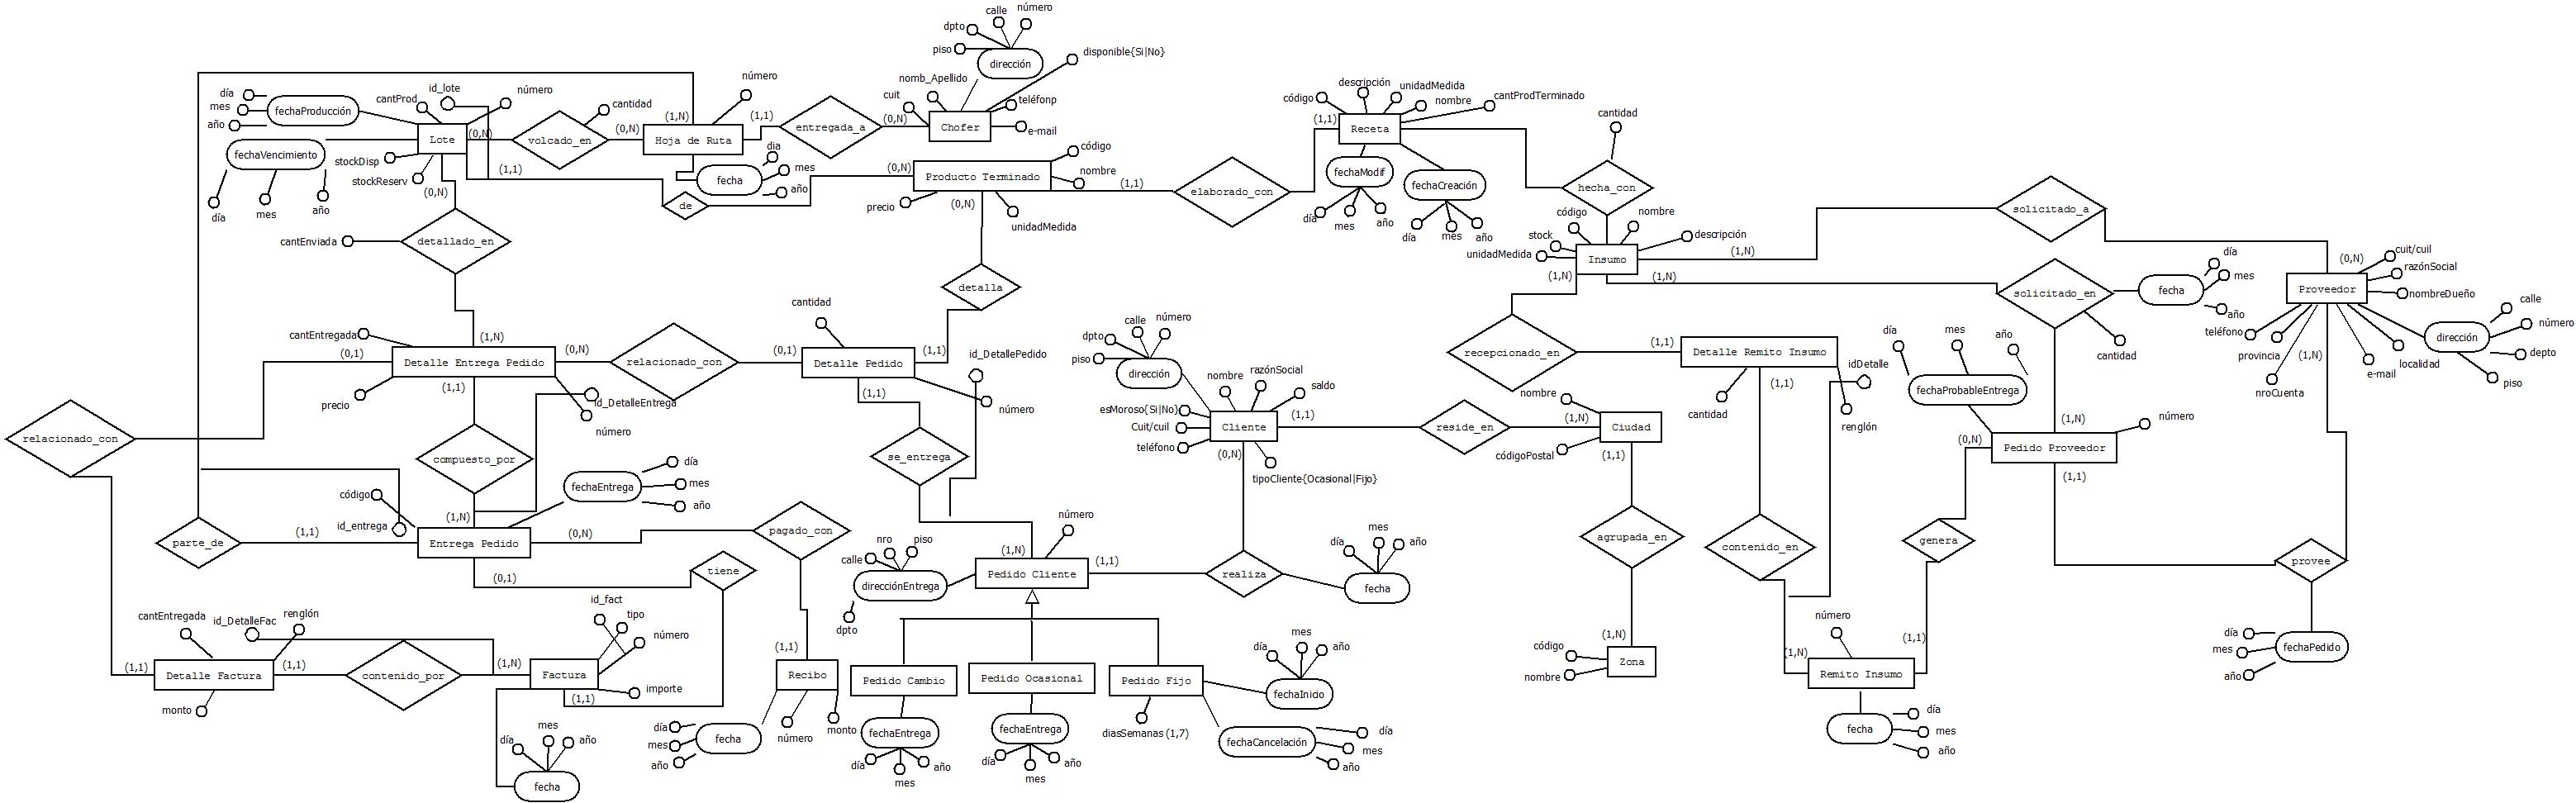
\includegraphics{modeloER.jpeg}


\section{Diagrama de clases}
\label{proyecto:diagrama-de-clases}
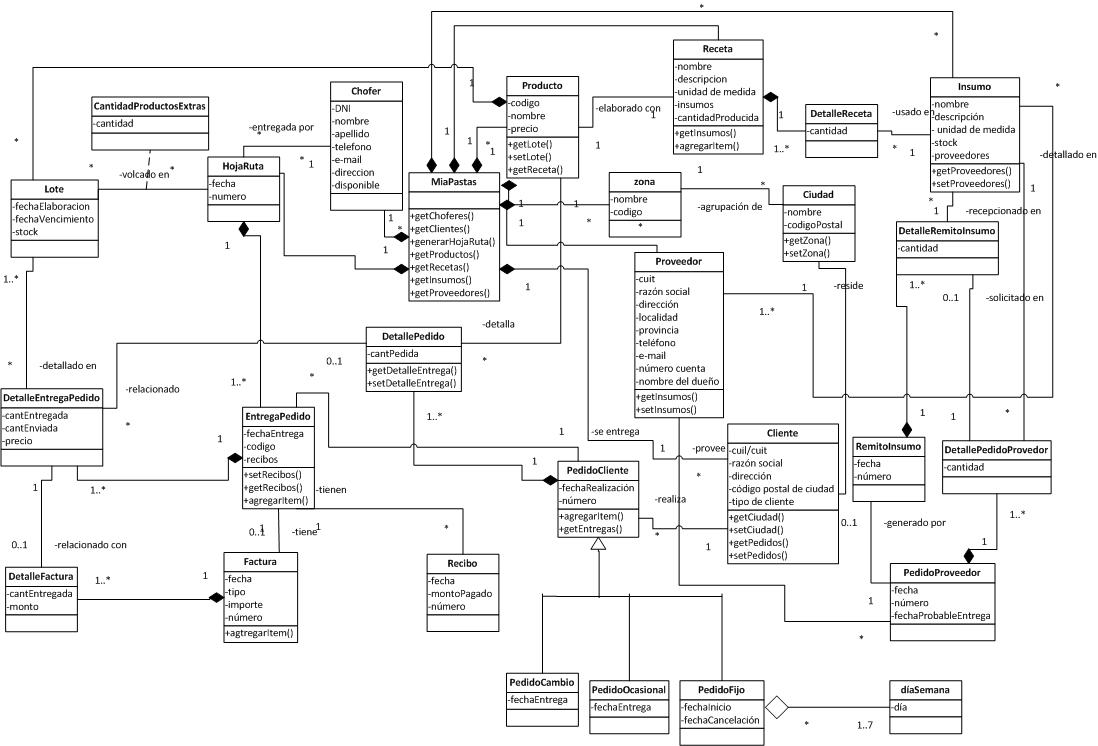
\includegraphics{DIAGRAMAClases.jpg}


\section{Diagrama de estados de pedido}
\label{proyecto:diagrama-de-estados-de-pedido}
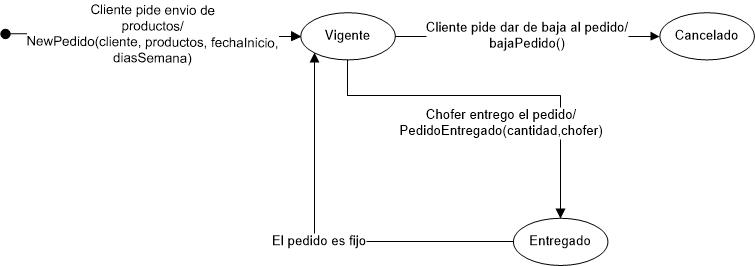
\includegraphics{diagramaEstadospedido.jpg}


\chapter{Codigo}
\label{codigo:codigo}\label{codigo::doc}

\section{Codigo de Recetas}
\label{codigo recetas:codigo-de-recetas}\label{codigo recetas::doc}\label{codigo recetas:module-recetas.models}\index{recetas.models (module)}\index{Chofer (class in recetas.models)}

\begin{fulllineitems}
\phantomsection\label{codigo recetas:recetas.models.Chofer}\pysiglinewithargsret{\strong{class }\code{recetas.models.}\bfcode{Chofer}}{\emph{id}, \emph{cuit}, \emph{nombre}, \emph{direccion}, \emph{telefono}, \emph{e\_mail}, \emph{activo}, \emph{disponible}}{}
\end{fulllineitems}

\index{Ciudad (class in recetas.models)}

\begin{fulllineitems}
\phantomsection\label{codigo recetas:recetas.models.Ciudad}\pysiglinewithargsret{\strong{class }\code{recetas.models.}\bfcode{Ciudad}}{\emph{id}, \emph{nombre}, \emph{codigo\_postal}, \emph{zona}}{}
\end{fulllineitems}

\index{Cliente (class in recetas.models)}

\begin{fulllineitems}
\phantomsection\label{codigo recetas:recetas.models.Cliente}\pysiglinewithargsret{\strong{class }\code{recetas.models.}\bfcode{Cliente}}{\emph{id}, \emph{cuit}, \emph{razon\_social}, \emph{nombre\_dueno}, \emph{ciudad}, \emph{direccion}, \emph{telefono}, \emph{email}, \emph{es\_moroso}, \emph{saldo}}{}
\end{fulllineitems}

\index{DetallePedidoProveedor (class in recetas.models)}

\begin{fulllineitems}
\phantomsection\label{codigo recetas:recetas.models.DetallePedidoProveedor}\pysiglinewithargsret{\strong{class }\code{recetas.models.}\bfcode{DetallePedidoProveedor}}{\emph{id}, \emph{cantidad\_insumo}, \emph{insumo}, \emph{pedido\_proveedor}}{}
\end{fulllineitems}

\index{Entrega (class in recetas.models)}

\begin{fulllineitems}
\phantomsection\label{codigo recetas:recetas.models.Entrega}\pysiglinewithargsret{\strong{class }\code{recetas.models.}\bfcode{Entrega}}{\emph{id}, \emph{hoja\_de\_ruta}, \emph{pedido}, \emph{fecha}, \emph{factura}}{}~\index{cobrar\_con\_factura() (recetas.models.Entrega method)}

\begin{fulllineitems}
\phantomsection\label{codigo recetas:recetas.models.Entrega.cobrar_con_factura}\pysiglinewithargsret{\bfcode{cobrar\_con\_factura}}{\emph{monto}, \emph{numero\_factura=None}}{}
recibe monto que debe coincidir con el precio total de la entrega
si resiba un nro de factura, asocia esa factura a la entrega.
si no recibe nro de factura, crea nueva factura y la asocia a la entrega

\end{fulllineitems}


\end{fulllineitems}

\index{EntregaDetalle (class in recetas.models)}

\begin{fulllineitems}
\phantomsection\label{codigo recetas:recetas.models.EntregaDetalle}\pysiglinewithargsret{\strong{class }\code{recetas.models.}\bfcode{EntregaDetalle}}{\emph{id}, \emph{entrega}, \emph{cantidad\_enviada}, \emph{cantidad\_entregada}, \emph{precio}, \emph{pedido\_cliente\_detalle}, \emph{producto\_terminado}}{}
\end{fulllineitems}

\index{Factura (class in recetas.models)}

\begin{fulllineitems}
\phantomsection\label{codigo recetas:recetas.models.Factura}\pysiglinewithargsret{\strong{class }\code{recetas.models.}\bfcode{Factura}}{\emph{id}, \emph{fecha}, \emph{numero}, \emph{monto\_pagado}}{}
\end{fulllineitems}

\index{HojaDeRuta (class in recetas.models)}

\begin{fulllineitems}
\phantomsection\label{codigo recetas:recetas.models.HojaDeRuta}\pysiglinewithargsret{\strong{class }\code{recetas.models.}\bfcode{HojaDeRuta}}{\emph{id}, \emph{fecha\_creacion}, \emph{chofer}, \emph{rendida}}{}
\end{fulllineitems}

\index{Insumo (class in recetas.models)}

\begin{fulllineitems}
\phantomsection\label{codigo recetas:recetas.models.Insumo}\pysiglinewithargsret{\strong{class }\code{recetas.models.}\bfcode{Insumo}}{\emph{id}, \emph{nombre}, \emph{descripcion}, \emph{stock}, \emph{unidad\_medida}, \emph{activo}}{}
\end{fulllineitems}

\index{Lote (class in recetas.models)}

\begin{fulllineitems}
\phantomsection\label{codigo recetas:recetas.models.Lote}\pysiglinewithargsret{\strong{class }\code{recetas.models.}\bfcode{Lote}}{\emph{nro\_lote}, \emph{fecha\_produccion}, \emph{fecha\_vencimiento}, \emph{cantidad\_producida}, \emph{stock\_disponible}, \emph{stock\_reservado}, \emph{producto\_terminado}}{}~\index{reservar\_stock() (recetas.models.Lote method)}

\begin{fulllineitems}
\phantomsection\label{codigo recetas:recetas.models.Lote.reservar_stock}\pysiglinewithargsret{\bfcode{reservar\_stock}}{\emph{cantidad}}{}
Resibe la cantidad de stock que se necesita reservar.
Si stock disponible alcanza a cubrirla, se aumenta el stock reservado en esa cantidad
Si stock disponible no alcanza a cubrirla, se aumenta el stock reservado con stock disponible
Este metodo retorna la cantidad que LOGRO reservar

\end{fulllineitems}


\end{fulllineitems}

\index{PedidoCambio (class in recetas.models)}

\begin{fulllineitems}
\phantomsection\label{codigo recetas:recetas.models.PedidoCambio}\pysiglinewithargsret{\strong{class }\code{recetas.models.}\bfcode{PedidoCambio}}{\emph{*args}, \emph{**kwargs}}{}
Clase que modela los pedidos de Cambio, es hija de PedidoCliente
Un pedido de cambio tiene fecha de entrega.
\index{esParaHoy() (recetas.models.PedidoCambio method)}

\begin{fulllineitems}
\phantomsection\label{codigo recetas:recetas.models.PedidoCambio.esParaHoy}\pysiglinewithargsret{\bfcode{esParaHoy}}{}{}
Metodo que verifica si un pedido tiene como fecha de entrega la fecha actual.

\end{fulllineitems}


\end{fulllineitems}

\index{PedidoCliente (class in recetas.models)}

\begin{fulllineitems}
\phantomsection\label{codigo recetas:recetas.models.PedidoCliente}\pysiglinewithargsret{\strong{class }\code{recetas.models.}\bfcode{PedidoCliente}}{\emph{*args}, \emph{**kwargs}}{}
Modelo de la clase padre de los pedidos de cliente
\index{esParaHoy() (recetas.models.PedidoCliente method)}

\begin{fulllineitems}
\phantomsection\label{codigo recetas:recetas.models.PedidoCliente.esParaHoy}\pysiglinewithargsret{\bfcode{esParaHoy}}{}{}
Metodo que los hijos lo redefinen

\end{fulllineitems}


\end{fulllineitems}

\index{PedidoClienteDetalle (class in recetas.models)}

\begin{fulllineitems}
\phantomsection\label{codigo recetas:recetas.models.PedidoClienteDetalle}\pysiglinewithargsret{\strong{class }\code{recetas.models.}\bfcode{PedidoClienteDetalle}}{\emph{*args}, \emph{**kwargs}}{}
Clase que modela los detalles de los pedidos independientemente del tipo (fijo, ocacional o de cambio)

\end{fulllineitems}

\index{PedidoFijo (class in recetas.models)}

\begin{fulllineitems}
\phantomsection\label{codigo recetas:recetas.models.PedidoFijo}\pysiglinewithargsret{\strong{class }\code{recetas.models.}\bfcode{PedidoFijo}}{\emph{*args}, \emph{**kwargs}}{}
Clase que modela los pedidos fijos, es hija de PedidoCliente
Un pedido fijo tiene fecha inicio, los dias para entregas los productos, y puede tener fecha de cancelacion
\index{esParaHoy() (recetas.models.PedidoFijo method)}

\begin{fulllineitems}
\phantomsection\label{codigo recetas:recetas.models.PedidoFijo.esParaHoy}\pysiglinewithargsret{\bfcode{esParaHoy}}{}{}
Metodo que verifica si un pedido tiene como fecha de entrega la fecha actual.
Se lo utiliza al armar una hoja de ruta.
Ademas, realiza una ``baja logica'' si el pedido fijo ya esta vencido (si se paso la fecha de canceacion).

\end{fulllineitems}


\end{fulllineitems}

\index{PedidoOcacional (class in recetas.models)}

\begin{fulllineitems}
\phantomsection\label{codigo recetas:recetas.models.PedidoOcacional}\pysiglinewithargsret{\strong{class }\code{recetas.models.}\bfcode{PedidoOcacional}}{\emph{*args}, \emph{**kwargs}}{}
Clase que modela los pedidos ocacionales, es hija de PedidoCliente
Un pedido ocacional tiene fecha de entrega.
\index{esParaHoy() (recetas.models.PedidoOcacional method)}

\begin{fulllineitems}
\phantomsection\label{codigo recetas:recetas.models.PedidoOcacional.esParaHoy}\pysiglinewithargsret{\bfcode{esParaHoy}}{}{}
Metodo que verifica si un pedido tiene como fecha de entrega la fecha actual.

\end{fulllineitems}


\end{fulllineitems}

\index{PedidoProveedor (class in recetas.models)}

\begin{fulllineitems}
\phantomsection\label{codigo recetas:recetas.models.PedidoProveedor}\pysiglinewithargsret{\strong{class }\code{recetas.models.}\bfcode{PedidoProveedor}}{\emph{id}, \emph{fecha\_realizacion}, \emph{fecha\_de\_entrega}, \emph{proveedor}, \emph{estado\_pedido}, \emph{descripcion}, \emph{fecha\_cancelacion}}{}
\end{fulllineitems}

\index{PerdidaStock (class in recetas.models)}

\begin{fulllineitems}
\phantomsection\label{codigo recetas:recetas.models.PerdidaStock}\pysiglinewithargsret{\strong{class }\code{recetas.models.}\bfcode{PerdidaStock}}{\emph{*args}, \emph{**kwargs}}{}
Clase que modela el suceso de decrementar el stock de un lote debido a una perdida (por rotura, vencimiento u otros)

\end{fulllineitems}

\index{ProductoTerminado (class in recetas.models)}

\begin{fulllineitems}
\phantomsection\label{codigo recetas:recetas.models.ProductoTerminado}\pysiglinewithargsret{\strong{class }\code{recetas.models.}\bfcode{ProductoTerminado}}{\emph{id}, \emph{nombre}, \emph{stock}, \emph{precio}, \emph{dias\_vigencia}, \emph{activo}}{}
\end{fulllineitems}

\index{ProductosLlevados (class in recetas.models)}

\begin{fulllineitems}
\phantomsection\label{codigo recetas:recetas.models.ProductosLlevados}\pysiglinewithargsret{\strong{class }\code{recetas.models.}\bfcode{ProductosLlevados}}{\emph{id}, \emph{cantidad\_pedida}, \emph{cantidad\_enviada}, \emph{producto\_terminado}, \emph{hoja\_de\_ruta}, \emph{precio}}{}~\index{generar\_detalles() (recetas.models.ProductosLlevados method)}

\begin{fulllineitems}
\phantomsection\label{codigo recetas:recetas.models.ProductosLlevados.generar_detalles}\pysiglinewithargsret{\bfcode{generar\_detalles}}{}{}
En base al producto y a la cantidad pedida, sale a buscarlo en los lotes
por cada lote que se necesite para satisfacer la cantidad pedida se crea un detalle asociado a el
junto con la cantidad que pudo sacarle a ese lote.

\end{fulllineitems}


\end{fulllineitems}

\index{ProductosLlevadosDetalle (class in recetas.models)}

\begin{fulllineitems}
\phantomsection\label{codigo recetas:recetas.models.ProductosLlevadosDetalle}\pysiglinewithargsret{\strong{class }\code{recetas.models.}\bfcode{ProductosLlevadosDetalle}}{\emph{id}, \emph{cantidad}, \emph{lote}, \emph{producto\_llevado}, \emph{cantidad\_sobrante}}{}
\end{fulllineitems}

\index{Proveedor (class in recetas.models)}

\begin{fulllineitems}
\phantomsection\label{codigo recetas:recetas.models.Proveedor}\pysiglinewithargsret{\strong{class }\code{recetas.models.}\bfcode{Proveedor}}{\emph{id}, \emph{razon\_social}, \emph{nombre\_dueno}, \emph{direccion}, \emph{email}, \emph{localidad}, \emph{numero\_cuenta}, \emph{provincia}, \emph{telefono}, \emph{cuit}}{}
\end{fulllineitems}

\index{Receta (class in recetas.models)}

\begin{fulllineitems}
\phantomsection\label{codigo recetas:recetas.models.Receta}\pysiglinewithargsret{\strong{class }\code{recetas.models.}\bfcode{Receta}}{\emph{id}, \emph{fecha\_creacion}, \emph{nombre}, \emph{descripcion}, \emph{cant\_prod\_terminado}, \emph{producto\_terminado}}{}
\end{fulllineitems}

\index{RecetaDetalle (class in recetas.models)}

\begin{fulllineitems}
\phantomsection\label{codigo recetas:recetas.models.RecetaDetalle}\pysiglinewithargsret{\strong{class }\code{recetas.models.}\bfcode{RecetaDetalle}}{\emph{id}, \emph{cantidad\_insumo}, \emph{insumo}, \emph{receta}}{}
\end{fulllineitems}

\index{Recibo (class in recetas.models)}

\begin{fulllineitems}
\phantomsection\label{codigo recetas:recetas.models.Recibo}\pysiglinewithargsret{\strong{class }\code{recetas.models.}\bfcode{Recibo}}{\emph{id}, \emph{entrega}, \emph{fecha}, \emph{numero}, \emph{monto\_pagado}}{}
\end{fulllineitems}

\index{Zona (class in recetas.models)}

\begin{fulllineitems}
\phantomsection\label{codigo recetas:recetas.models.Zona}\pysiglinewithargsret{\strong{class }\code{recetas.models.}\bfcode{Zona}}{\emph{id}, \emph{nombre}}{}
\end{fulllineitems}



\section{Codigo de Zonas}
\label{codigo zonas:codigo-de-zonas}\label{codigo zonas::doc}

\section{Codigo de Clientes}
\label{codigo clientes:codigo-de-clientes}\label{codigo clientes::doc}

\chapter{{}AYUDA DE USUARIO}
\label{ayuda usuario::doc}\label{ayuda usuario:ayuda-de-usuario}

\section{Ayuda}
\label{ayuda usuario:ayuda}

\subsection{{}Recetas}
\label{recetas::doc}\label{recetas:recetas}
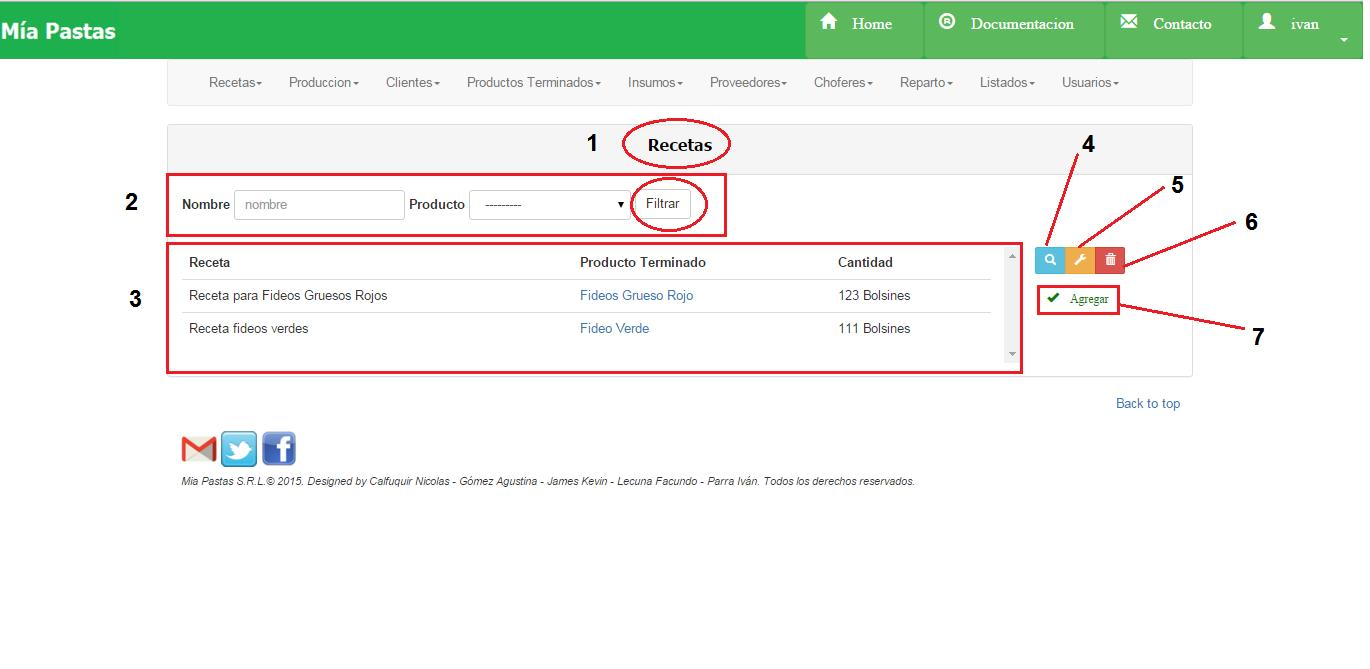
\includegraphics{rece_ini.jpg}
\begin{enumerate}
\item {} 
Nombre de la sección donde estamos ubicados.

\item {} 
Es el sector de filtrado, se podrá filtrar por nombre o producto.

\item {} 
Área de resultado del filtro donde se mostrará nombre, producto terminado y cantidad, de no haberse realizado ningún filtro mostrará todas las recetas existentes. Al hacer click en Producto terminado mostrará todos los datos del producto terminado asociado.

\item {} 
El icono de lupa sirve para mostrar más detalle sobre el ítem seleccionado como se muestra en la siguiente figura. De no seleccionar previamente un ítem aparecerá un mensaje de error.

\item {} 
El icono de llave sirve para realizar una modificación sobre el ítem seleccionado. Para esto se deberá hacer click previamente sobre el ítem deseado. De no seleccionar previamente un ítem aparecerá un mensaje de error.

\item {} 
Eliminar una receta.

\item {} 
Alta de una receta, permite crear una receta.

\end{enumerate}


\subsubsection{Consultar Recetas}
\label{recetas:consultar-recetas}
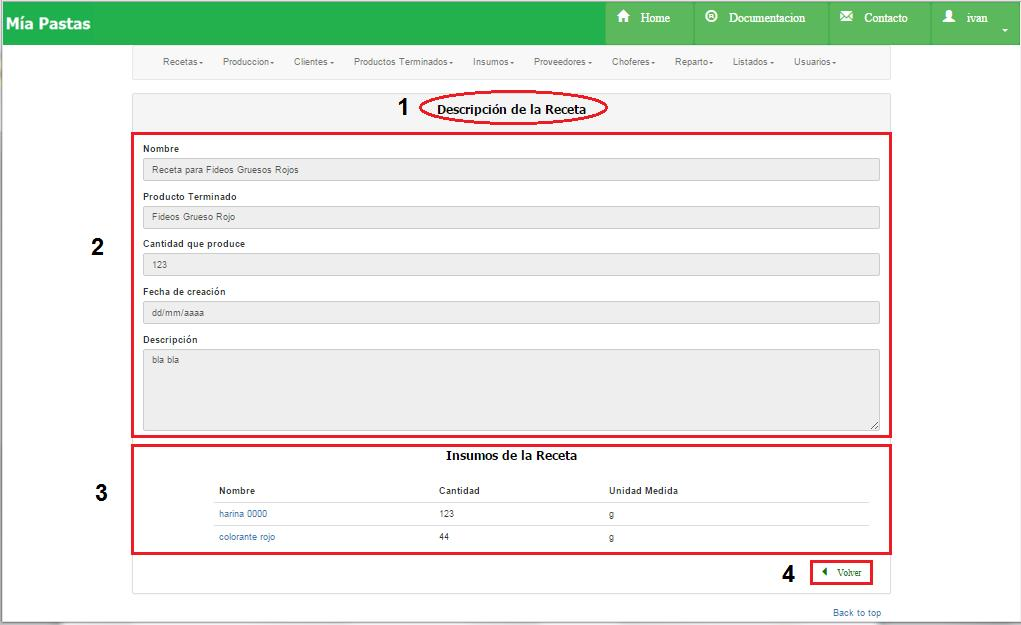
\includegraphics{receta_detalle.jpg}
\begin{enumerate}
\item {} 
Nombre de la sección en la que nos ubicamos, (2) descripción de la receta, (3) el detalle de la receta, (4) botón para volver a la página anterior.

\end{enumerate}


\subsubsection{Modificar Recetas}
\label{recetas:modificar-recetas}
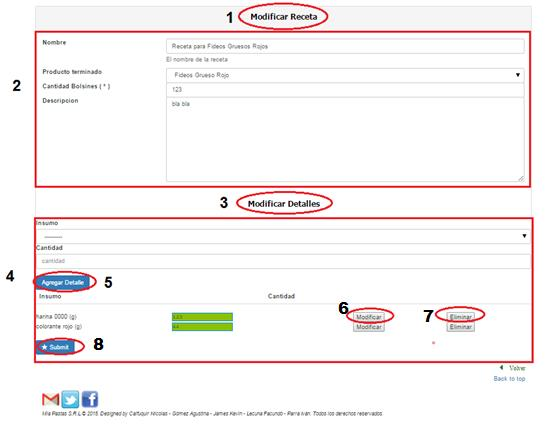
\includegraphics{receta_modificar.jpg}
\begin{enumerate}
\item {} 
Nombre de la sección en la que nos ubicamos, (2) descripción de la receta a modificar, (3 y 4) el detalle de la receta a modificar, (5) agregar un insumo y su cantidad a la receta, (6) modificar la cantidad del insumo, (7) eliminar el insumo de la receta, (8) guardar los cambios de la receta.

\end{enumerate}


\subsubsection{Eliminar Recetas}
\label{recetas:eliminar-recetas}
Se deberá seleccionar una receta haciendo click, y luego hacer click sobre el botón de eliminar. Aparecerá el siguiente cartel:

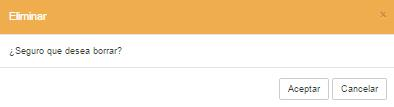
\includegraphics{receta_eliminar.jpg}


\subsubsection{Alta de Recetas}
\label{recetas:alta-de-recetas}
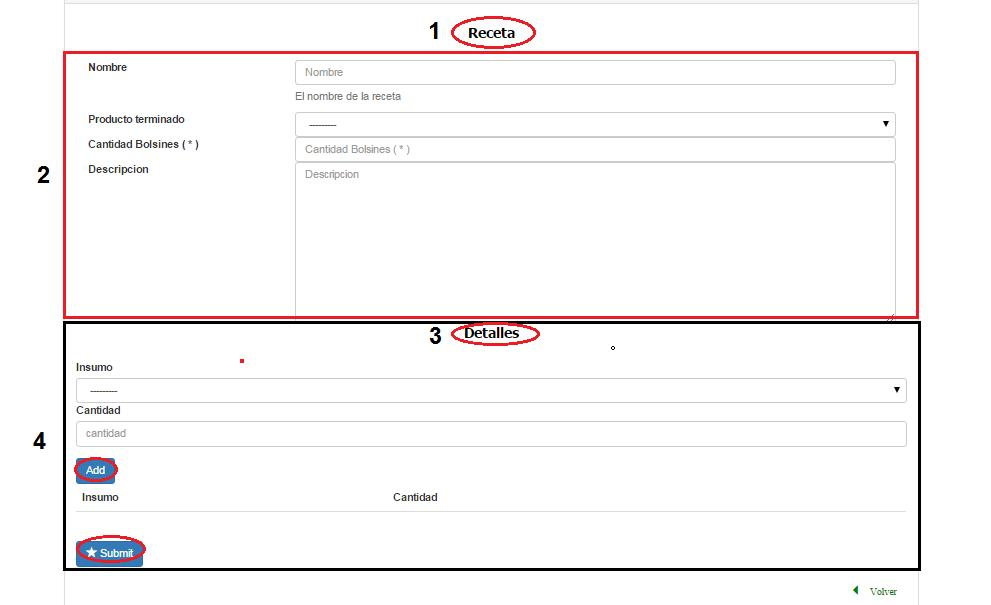
\includegraphics{receta_alta.jpg}
\begin{enumerate}
\item {} 
Nombre de la sección en la que nos ubicamos, (2) descripción de la receta a crear, (3 y 4) el detalle de la receta a crear, agregar un insumo y su cantidad a la receta,  debajo se encuentra el botón de guardar.

\end{enumerate}


\paragraph{{}Consultar Recetas}
\label{recetas consultar::doc}\label{recetas consultar:consultar-recetas}
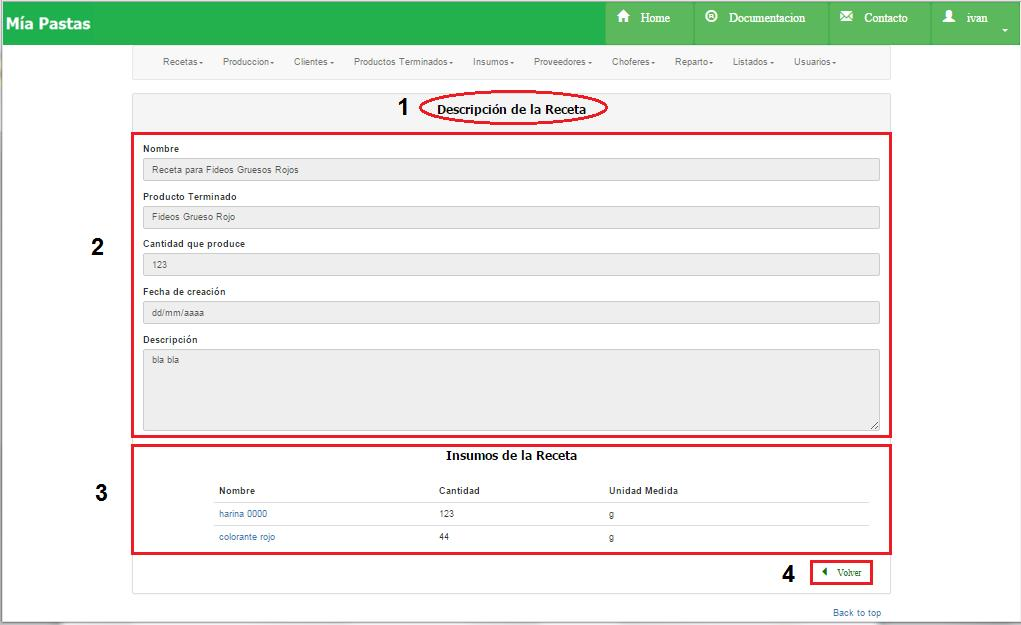
\includegraphics{receta_detalle.jpg}
\begin{enumerate}
\item {} 
Nombre de la sección en la que nos ubicamos, (2) descripción de la receta, (3) el detalle de la receta, (4) botón para volver a la página anterior.

\end{enumerate}


\paragraph{{}Alta Receta}
\label{recetas alta::doc}\label{recetas alta:alta-receta}
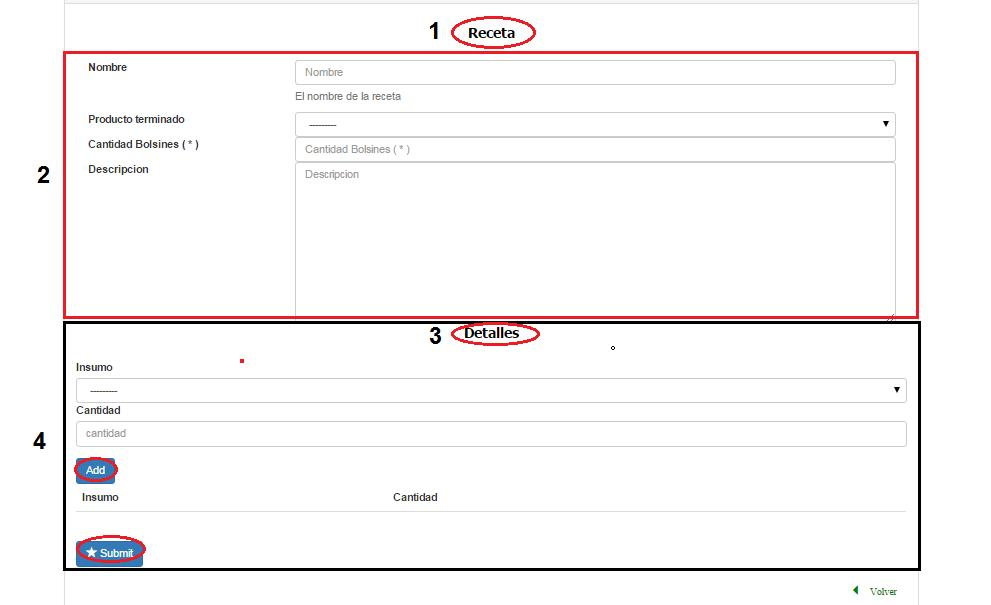
\includegraphics{receta_alta.jpg}
\begin{enumerate}
\item {} 
Nombre de la sección en la que nos ubicamos, (2) descripción de la receta a crear, (3 y 4) el detalle de la receta a crear, agregar un insumo y su cantidad a la receta,  debajo se encuentra el botón de guardar.

\end{enumerate}


\paragraph{{}Eliminar Receta}
\label{receta eliminar::doc}\label{receta eliminar:eliminar-receta}

\subsection{{}Producción}
\label{lotes:produccion}\label{lotes::doc}
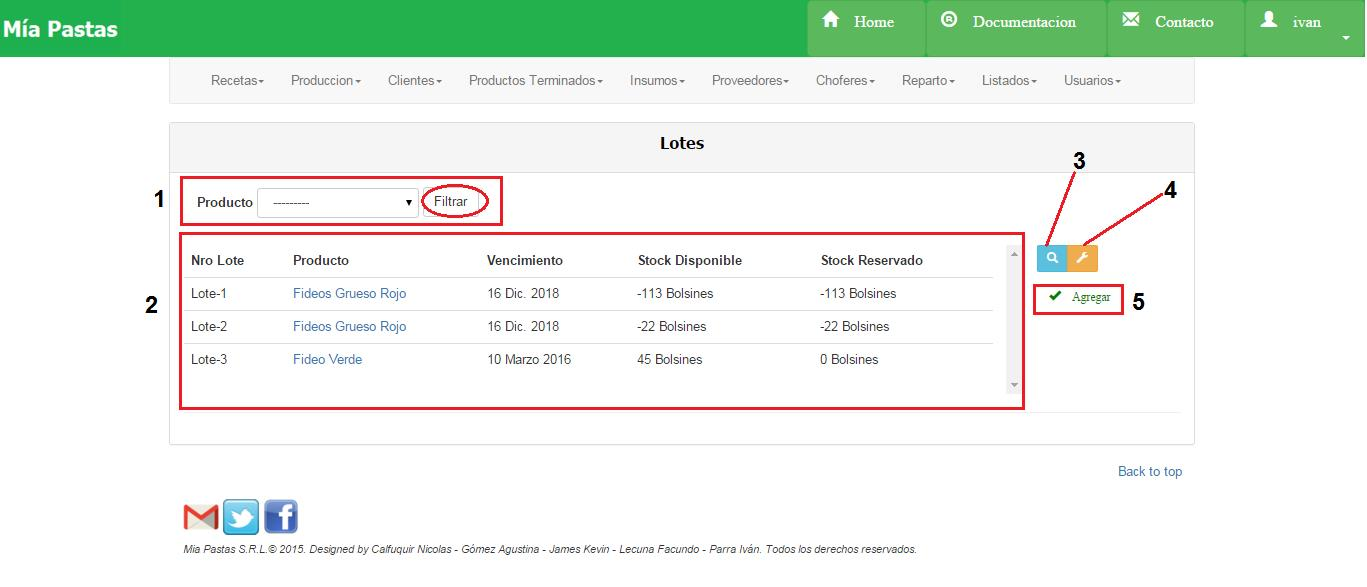
\includegraphics{lotes_ini.jpg}
\begin{enumerate}
\item {} 
Es el sector de filtrado, se podrá filtrar por tipo de producto.

\item {} 
Área de resultado del filtro donde se mostrará número de lote, nombre del producto vencimiento, stock disponible, stock reservado. De no haberse realizado ningún filtro mostrará todas las recetas existentes. Al hacer click en Producto mostrará todos los datos del producto terminado asociado.

\item {} 
El icono de lupa sirve para mostrar más detalle sobre el ítem seleccionado. De no seleccionar previamente un ítem aparecerá un mensaje de error.

\item {} 
El icono de llave sirve para realizar una modificación sobre el ítem seleccionado. Para esto se deberá hacer click previamente sobre el ítem deseado. De no seleccionar previamente un ítem aparecerá un mensaje de error.

\item {} 
Registrar una Nueva Producción.

\end{enumerate}


\subsubsection{Consultar Lote}
\label{lotes:consultar-lote}
Seleccionar un lote haciendo click sobre el deseado y sobre el ícono de lupa.

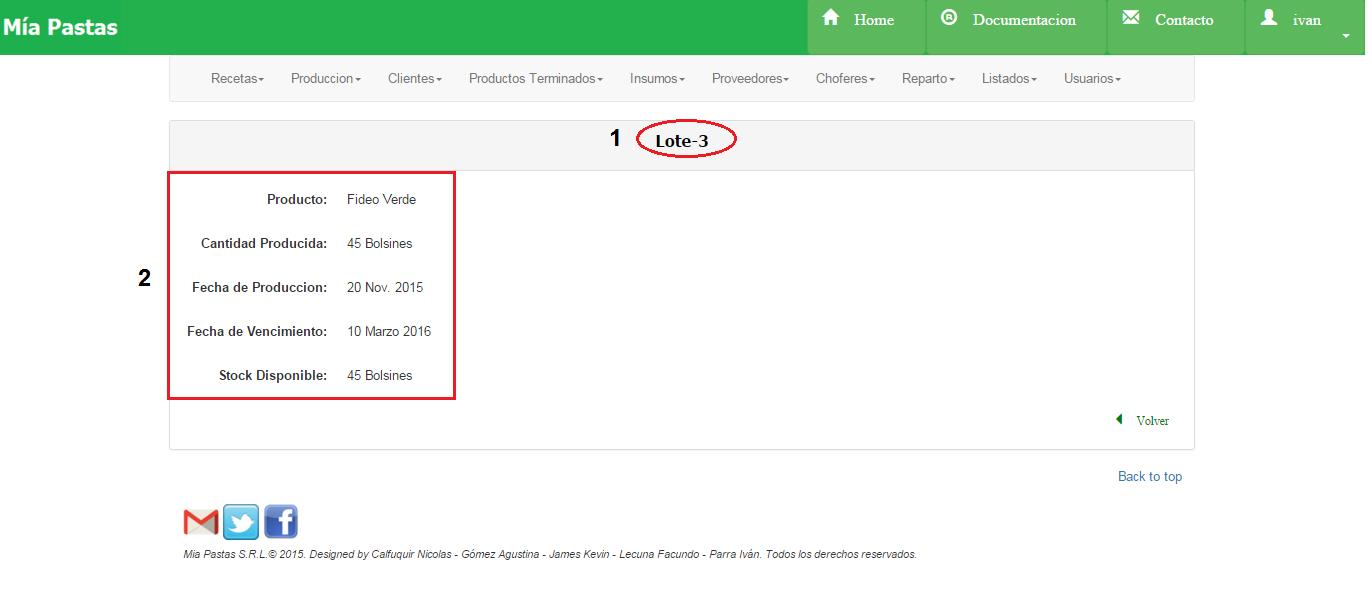
\includegraphics{lotes_detalle.jpg}

Como vemos, en (1) vemos el nombre del Lote seleccionado, y en la sección (2) vemos los datos de ese lote.


\subsubsection{Modificar Stock de Lote}
\label{lotes:modificar-stock-de-lote}
Seleccionar con un click el lote a modificar stock, luego hacer click sobre el ícono de modificar.

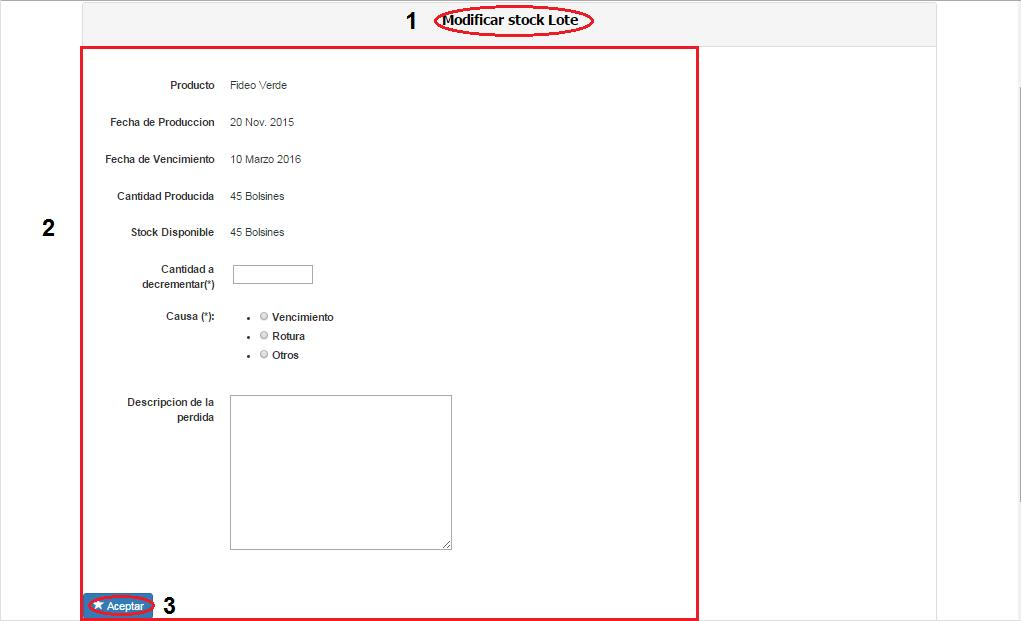
\includegraphics{lotes_modificar.jpg}
\begin{enumerate}
\item {} 
Nombre de la sección en la que nos ubicamos, (2) descripción del lote a modificar, (3) guardar los cambios del lote.

\end{enumerate}


\subsubsection{Alta Lote}
\label{lotes:alta-lote}
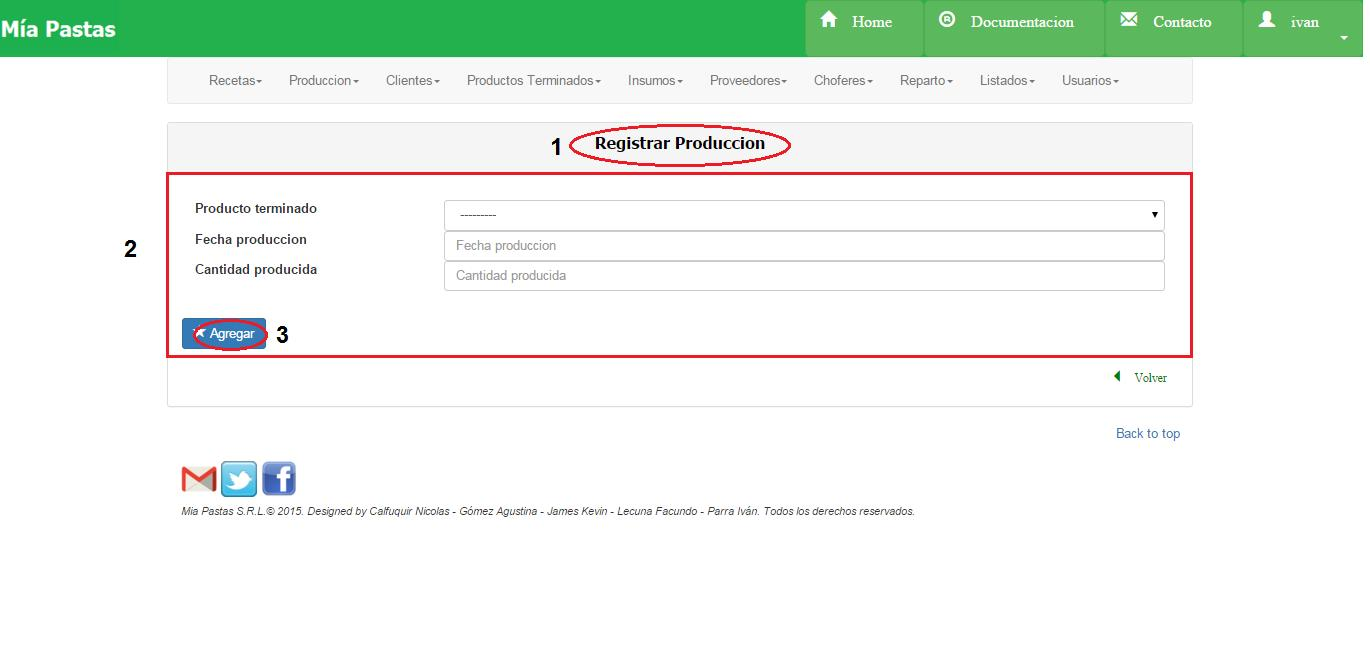
\includegraphics{lotes_alta.jpg}
\begin{enumerate}
\item {} 
Nombre de la sección en la que nos ubicamos, (2) descripción del lote a crear, (3) botón de guardar.

\end{enumerate}


\paragraph{{}Consultar Lotes}
\label{lotes consultar:consultar-lotes}\label{lotes consultar::doc}
Seleccionar un lote haciendo click sobre el deseado y sobre el ícono de lupa.

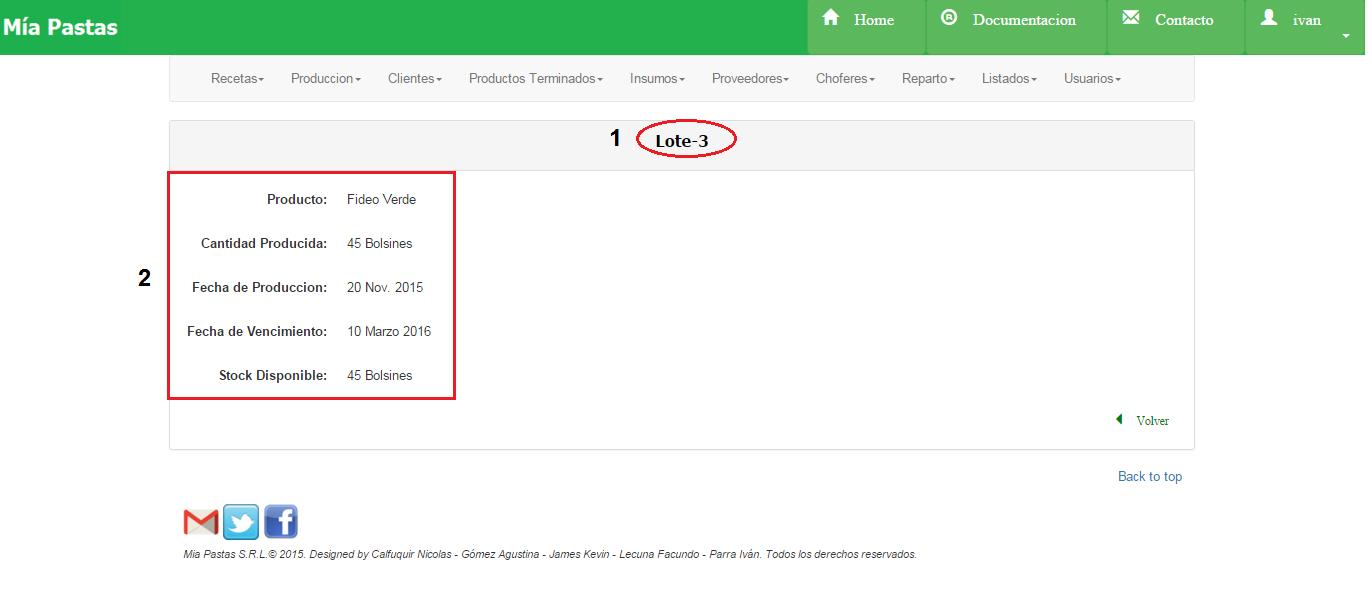
\includegraphics{lotes_detalle.jpg}

Como vemos, en (1) vemos el nombre del Lote seleccionado, y en la sección (2) vemos los datos de ese lote.


\paragraph{{}Lotes alta}
\label{lotes alta::doc}\label{lotes alta:lotes-alta}
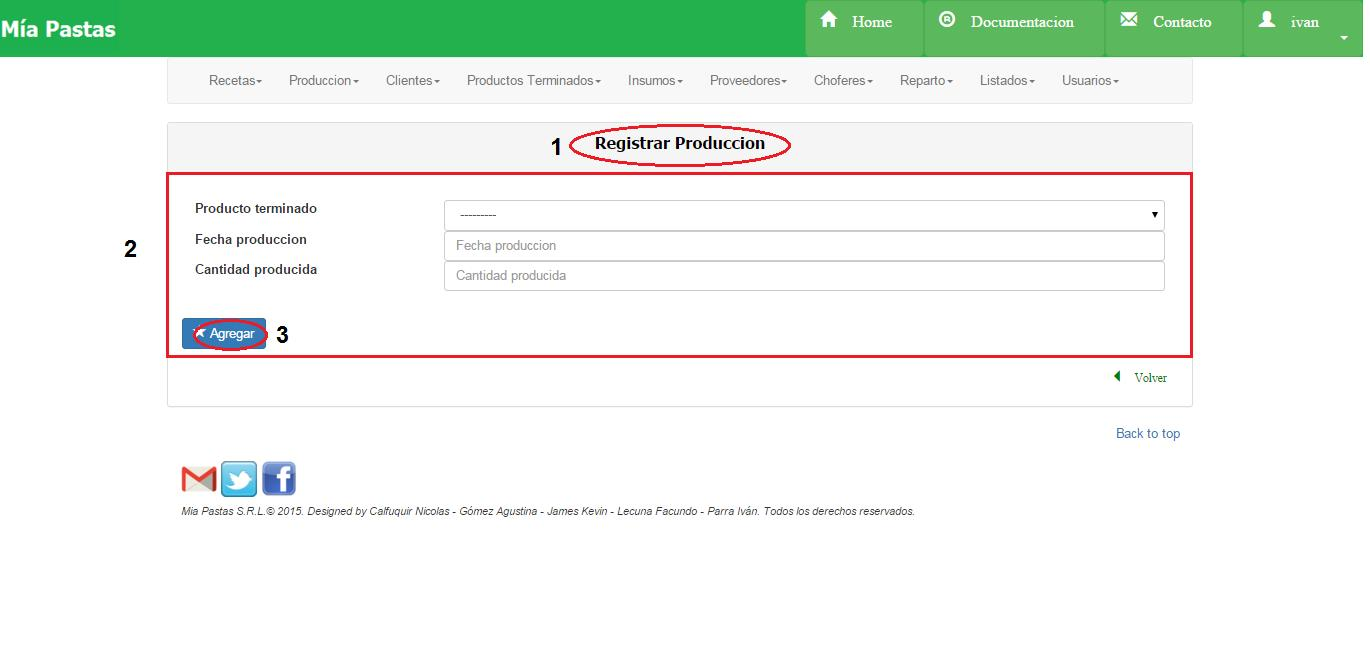
\includegraphics{lotes_alta.jpg}
\begin{enumerate}
\item {} 
Nombre de la sección en la que nos ubicamos, (2) descripción del lote a crear, (3) botón de guardar.

\end{enumerate}


\paragraph{{}Modificar Stock de Lote}
\label{productosTerminadosActualizarStock consultar::doc}\label{productosTerminadosActualizarStock consultar:modificar-stock-de-lote}
Seleccionar con un click el lote a modificar stock, luego hacer click sobre el ícono de modificar.

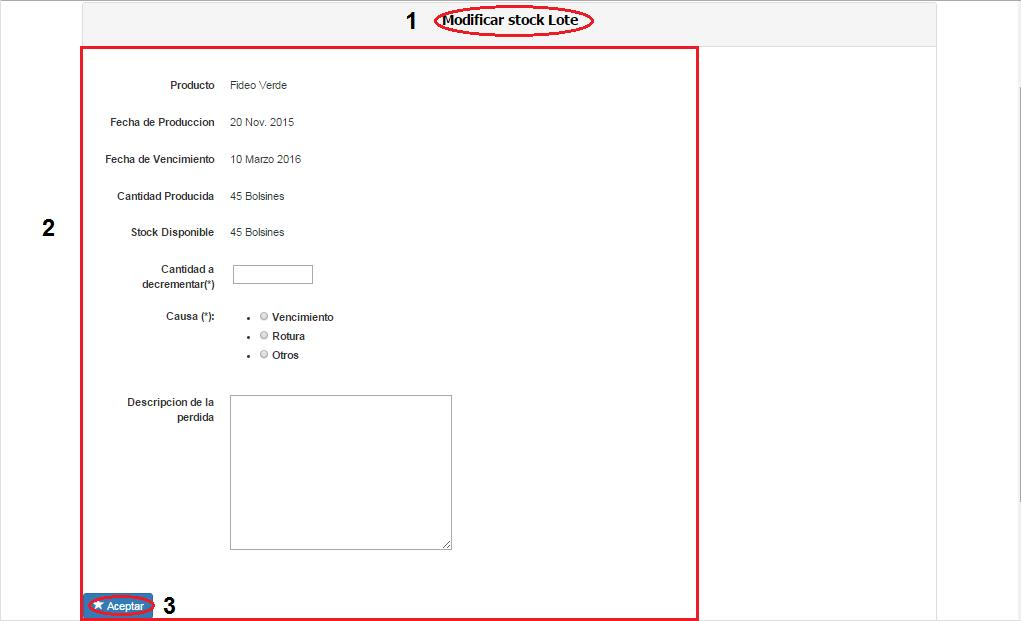
\includegraphics{lotes_modificar.jpg}
\begin{enumerate}
\item {} 
Nombre de la sección en la que nos ubicamos, (2) descripción del lote a modificar, (3) guardar los cambios del lote.

\end{enumerate}


\subsection{{}Cobrar Cliente}
\label{cobrarCliente:cobrar-cliente}\label{cobrarCliente::doc}

\subsubsection{Pantalla Principal de Cobrar Clientes}
\label{cobrarCliente:pantalla-principal-de-cobrar-clientes}
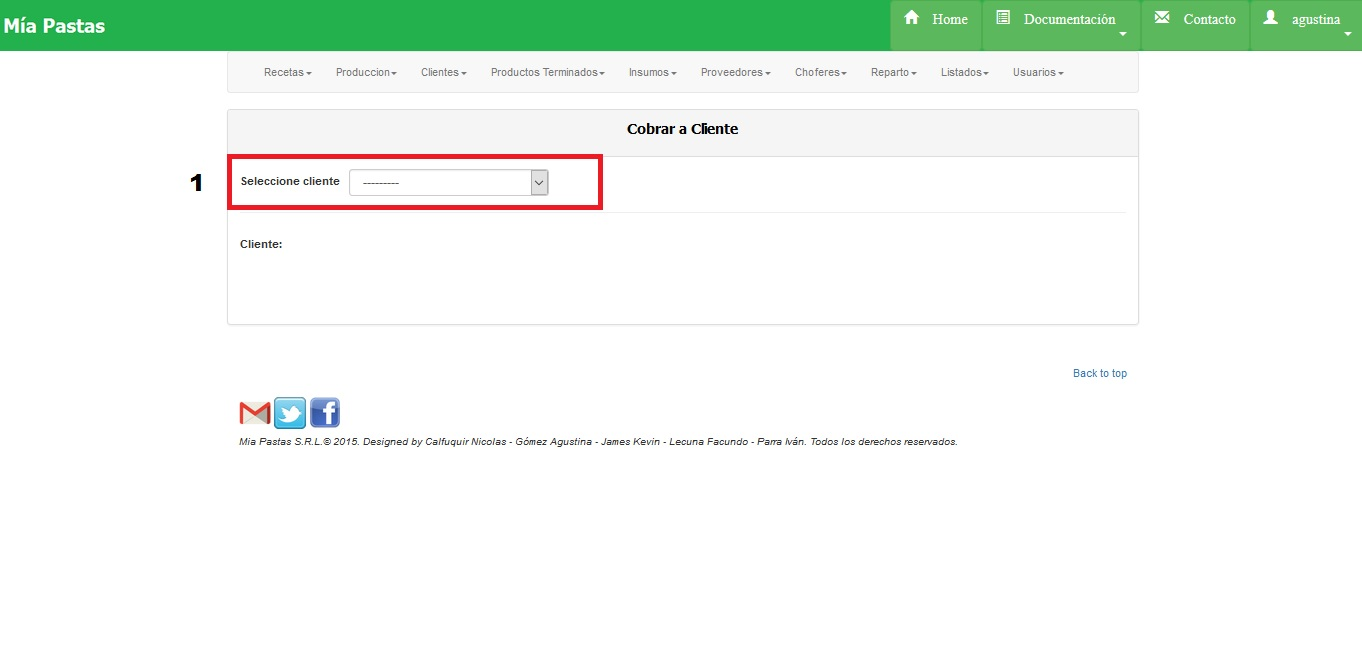
\includegraphics{cobrar_ini.jpg}
\begin{enumerate}
\item {} 
Es el sector de filtrado, se podrá filtrar por nombre del cliente

\end{enumerate}


\subsubsection{Consultar Clientes}
\label{cobrarCliente:consultar-clientes}
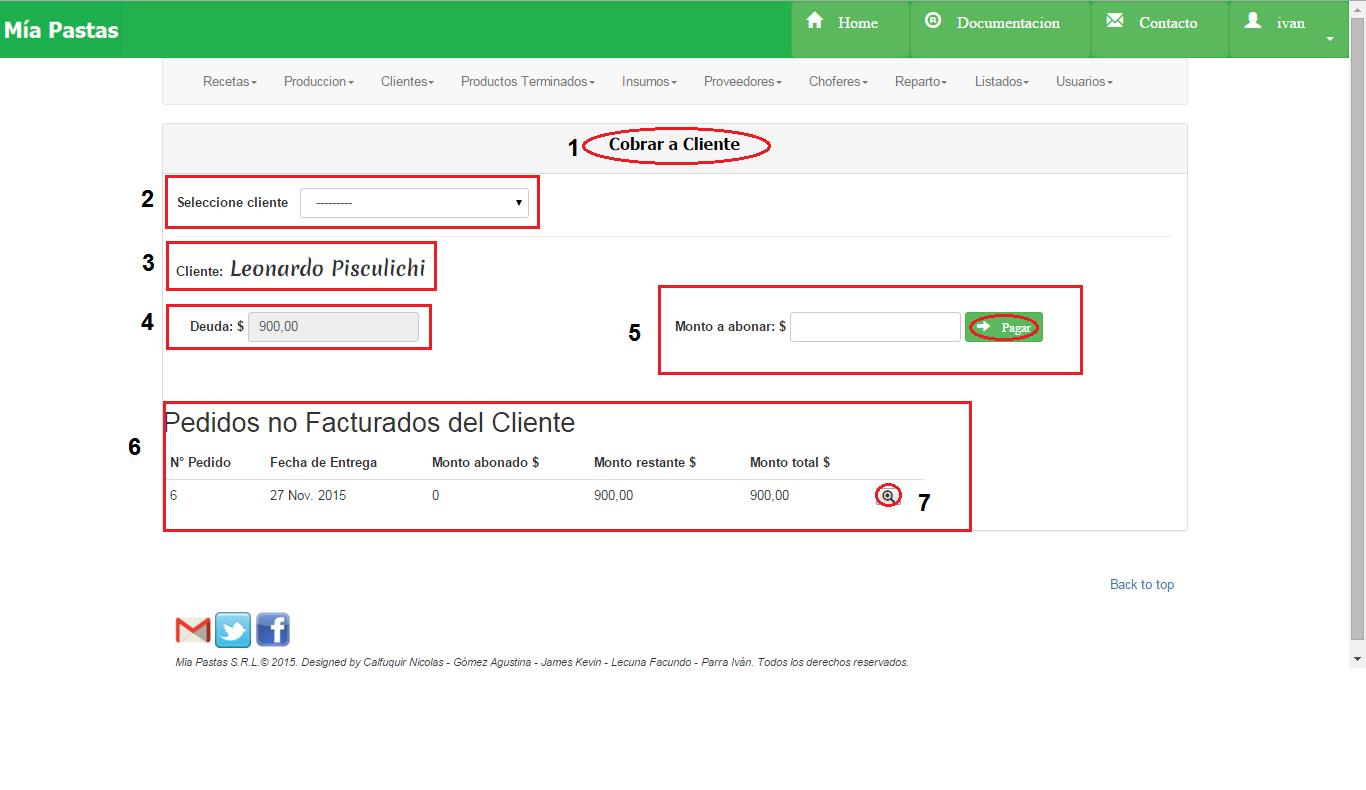
\includegraphics{cobrar.jpg}
\begin{enumerate}
\item {} 
Nombre de la sección donde estamos ubicados.

\item {} 
Es el sector de filtrado, se podrá filtrar por nombre de cliente.

\item {} 
Muestra nombre del cliente seleccionado.

\item {} 
Área de resultado del filtro donde se mostrará la deuda total del cliente

\item {} 
Área donde se debe indicar el monto a abonar por el cliente, el botón pagar efectúa la confirmación del pago.

\item {} 
Área que muestra los pedidos adeudados por el cliente. Indica número de pedido, fecha de Entrega, Monto abonado (parcial), monto restante y monto total. (7) Con la lupa se mostrará el detalle del pedido seleccionado.

\end{enumerate}


\paragraph{{}Consultar Clientes}
\label{cobrarCliente consultarFiltrad::doc}\label{cobrarCliente consultarFiltrad:consultar-clientes}
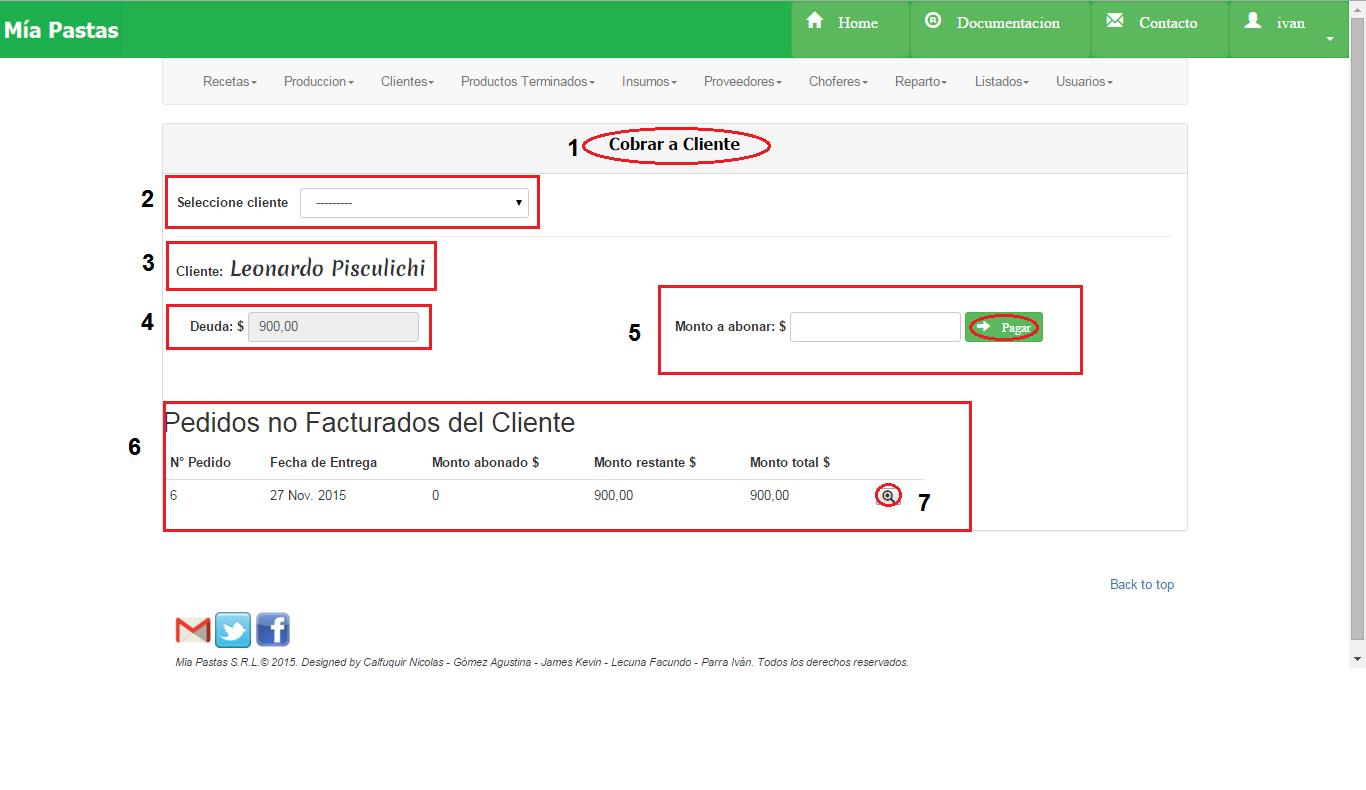
\includegraphics{cobrar.jpg}
\begin{enumerate}
\item {} 
Nombre de la sección donde estamos ubicados.

\item {} 
Es el sector de filtrado, se podrá filtrar por nombre de cliente.

\item {} 
Muestra nombre del cliente seleccionado.

\item {} 
Área de resultado del filtro donde se mostrará la deuda total del cliente

\item {} 
Área donde se debe indicar el monto a abonar por el cliente, el botón pagar efectúa la confirmación del pago.

\item {} 
Área que muestra los pedidos adeudados por el cliente. Indica número de pedido, fecha de Entrega, Monto abonado (parcial), monto restante y monto total. (7) Con la lupa se mostrará el detalle del pedido seleccionado.

\end{enumerate}


\subsection{{}Ciudades}
\label{ciudades:ciudades}\label{ciudades::doc}
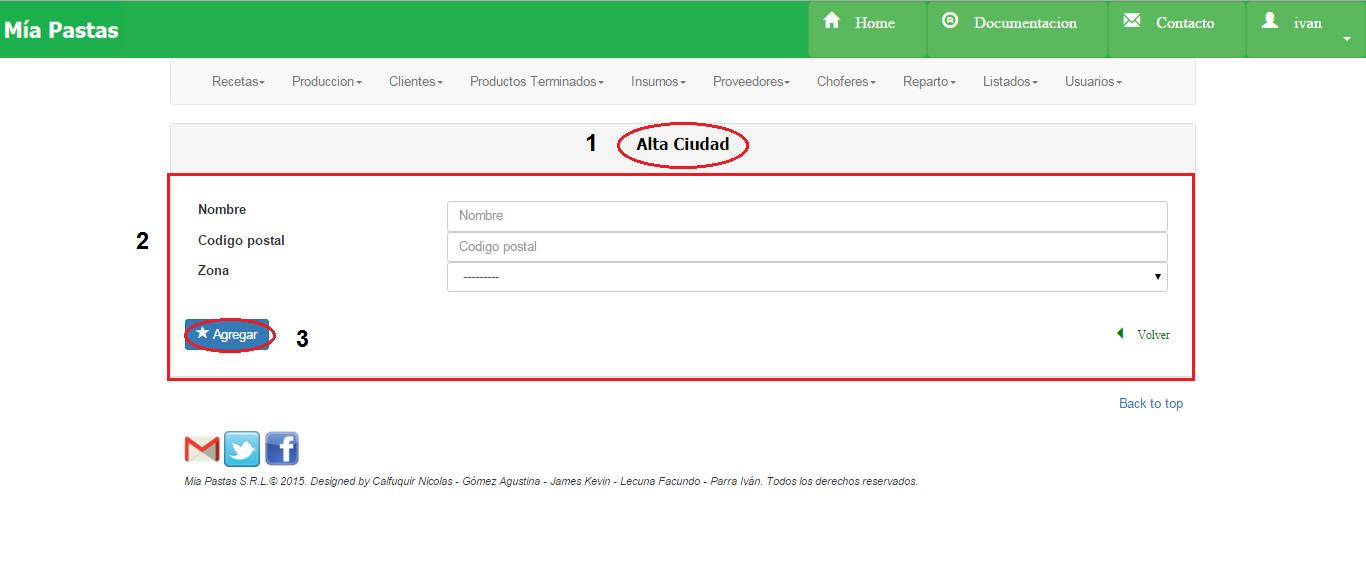
\includegraphics{ciudades_alta.jpg}
\begin{enumerate}
\item {} 
Nombre de la sección donde estamos ubicados.

\end{enumerate}

2.      Es el sector de filtrado, se podrá filtrar por nombre, código postal, zona. Se filtrará presionando el botón (3).
4.      Área de resultado del filtro donde se mostrará nombre, código postal y zona de las ciudades filtradas. De no haberse realizado ningún filtro mostrará todos los clientes existentes. Al hacer click en Zona mostrará todos los datos de la zona asociada.
5.      El icono de lupa sirve para mostrar más detalle sobre el ítem seleccionado como se muestra en la siguiente figura. De no seleccionar previamente un ítem aparecerá un mensaje de error.
6.      El icono de llave sirve para realizar una modificación sobre el ítem seleccionado. Para esto se deberá hacer click previamente sobre el ítem deseado. De no seleccionar previamente un ítem aparecerá un mensaje de error.
7.      Eliminar una ciudad.
8.      Dar de Alta una nueva ciudad


\subsubsection{Consultar Ciudades}
\label{ciudades:consultar-ciudades}
Seleccionar una ciudad click sobre el deseado y sobre el ícono de lupa.

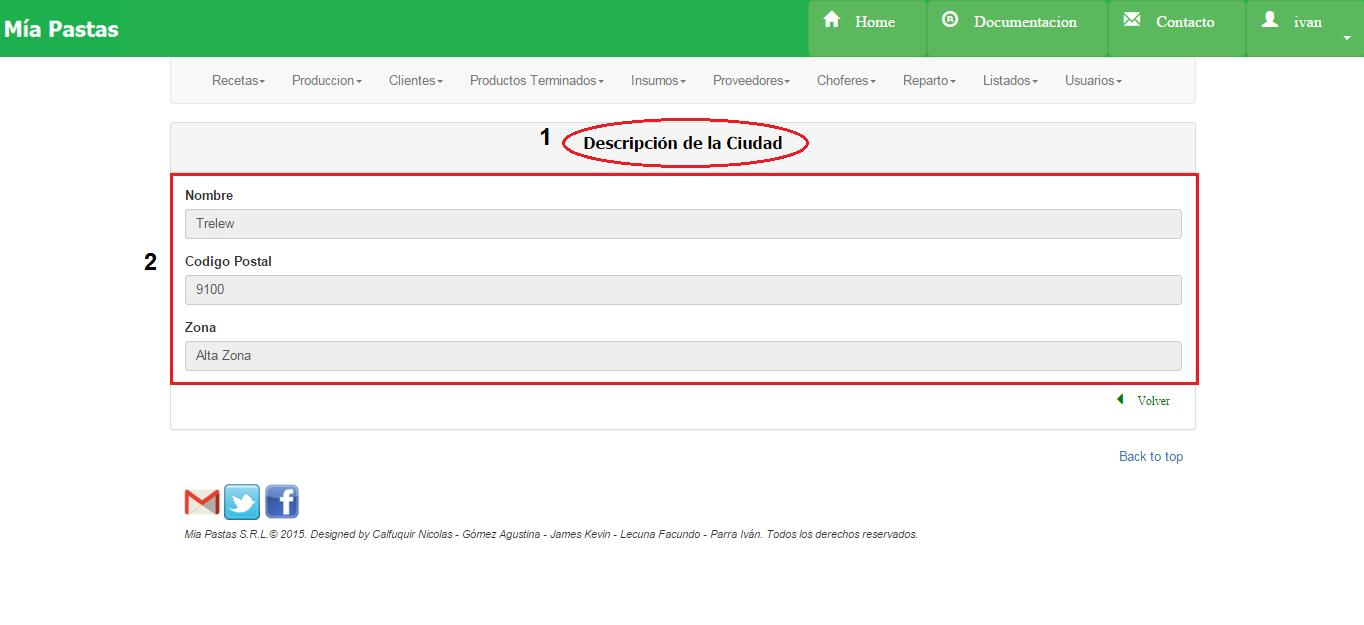
\includegraphics{ciudades_detalle.jpg}
\begin{enumerate}
\item {} 
Nombre de la sección en la que nos ubicamos, (2) descripción de la ciudad consultada.

\end{enumerate}


\subsubsection{Modificar Ciudades}
\label{ciudades:modificar-ciudades}
Seleccionar con un click la ciudad a modificar, luego hacer click sobre el ícono de modificar.

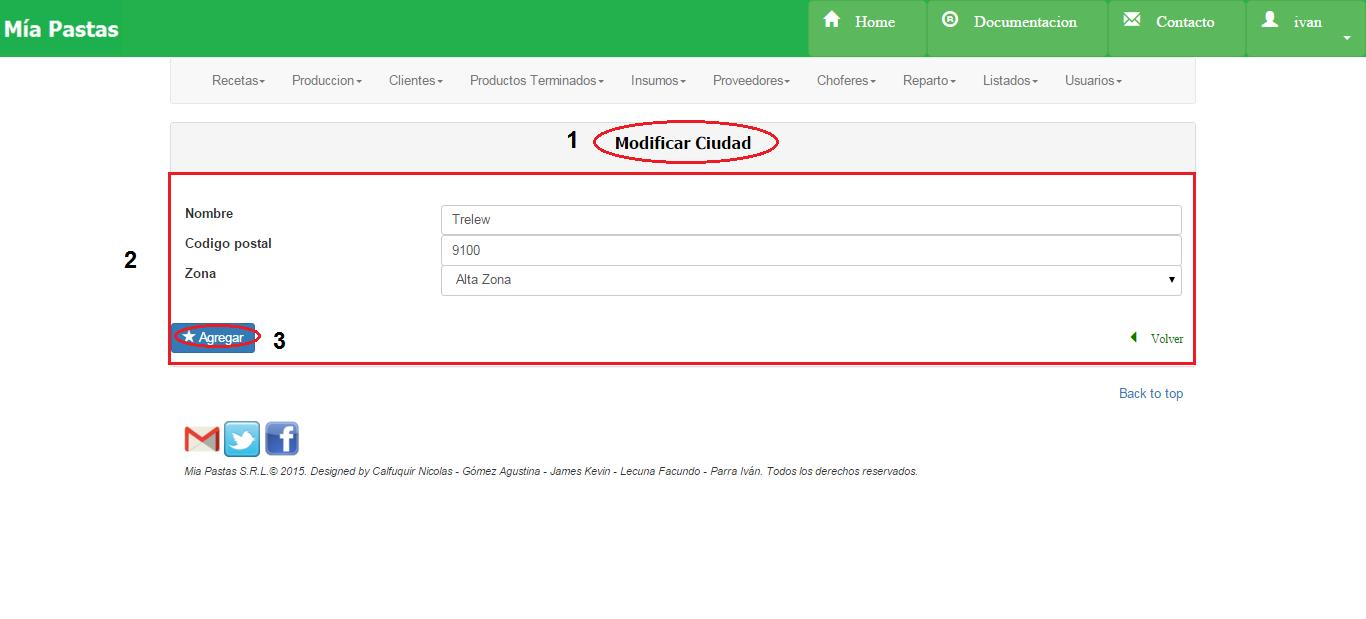
\includegraphics{ciudades_modificar.jpg}
\begin{enumerate}
\item {} 
Nombre de la sección en la que nos ubicamos, (2) descripción de la ciudad a modificar, (3)  guardar los cambios de la ciudad.

\end{enumerate}


\subsubsection{Alta Ciudad}
\label{ciudades:alta-ciudad}
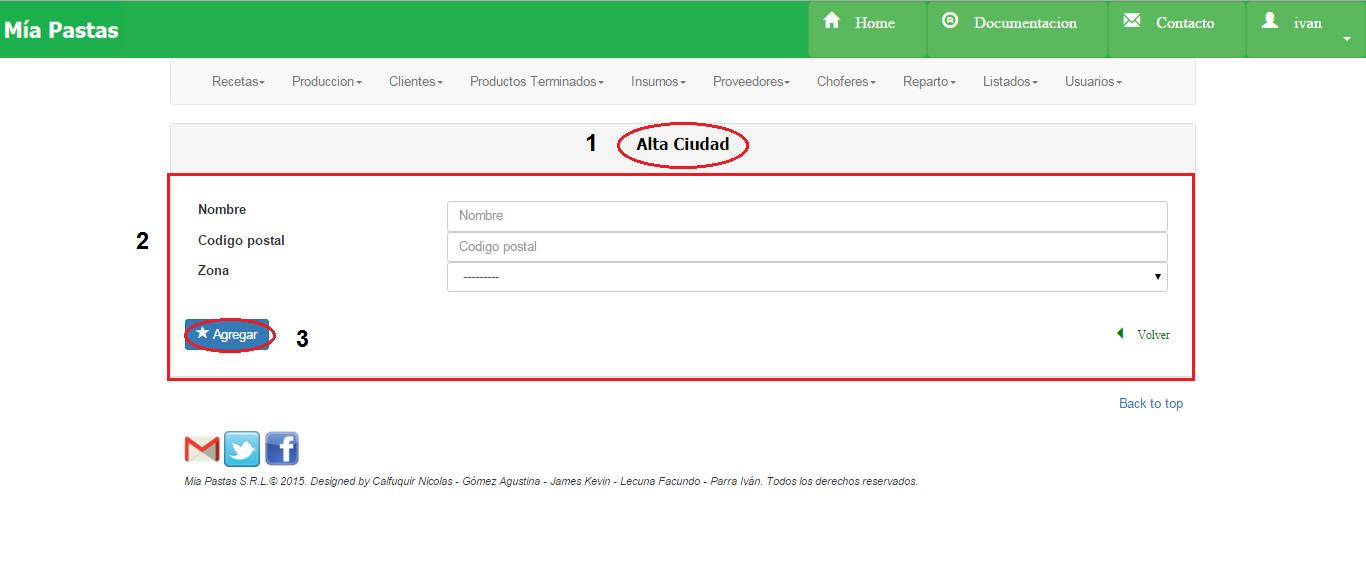
\includegraphics{ciudades_alta.jpg}
\begin{enumerate}
\item {} 
Nombre de la sección en la que nos ubicamos, (2) datos de la ciudad a crear, (3) confirmar el alta de nueva ciudad.

\end{enumerate}


\subsubsection{Eliminar Ciudades}
\label{ciudades:eliminar-ciudades}
Seleccionar con click una ciudad y hacer click sobre el botón de eliminar. Aparecerá el siguiente cartel:

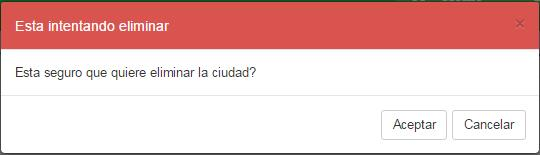
\includegraphics{ciudades_eliminar.jpg}

La ciudad no deberá tener clientes asociados


\paragraph{{}Consultar Ciudades}
\label{ciudades consultar:consultar-ciudades}\label{ciudades consultar::doc}
Seleccionar una ciudad click sobre el deseado y sobre el ícono de lupa.

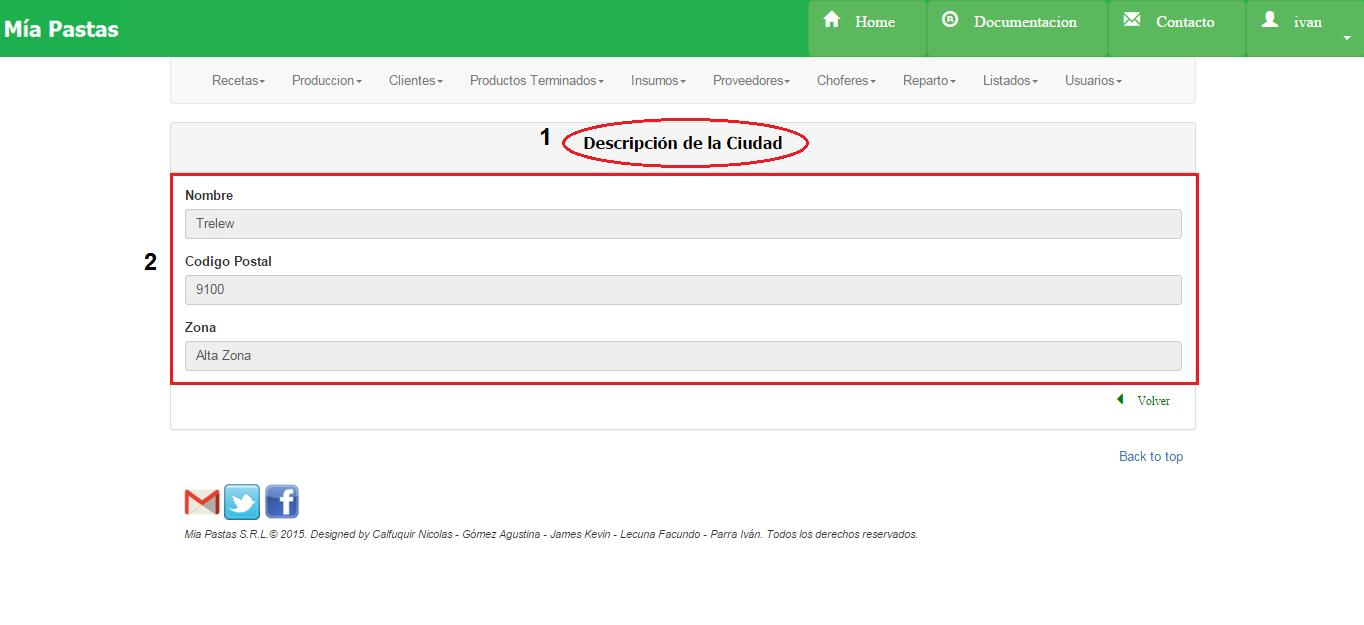
\includegraphics{ciudades_detalle.jpg}
\begin{enumerate}
\item {} 
Nombre de la sección en la que nos ubicamos, (2) descripción de la ciudad consultada.

\end{enumerate}


\paragraph{{}Alta Ciudad}
\label{ciudades alta:alta-ciudad}\label{ciudades alta::doc}
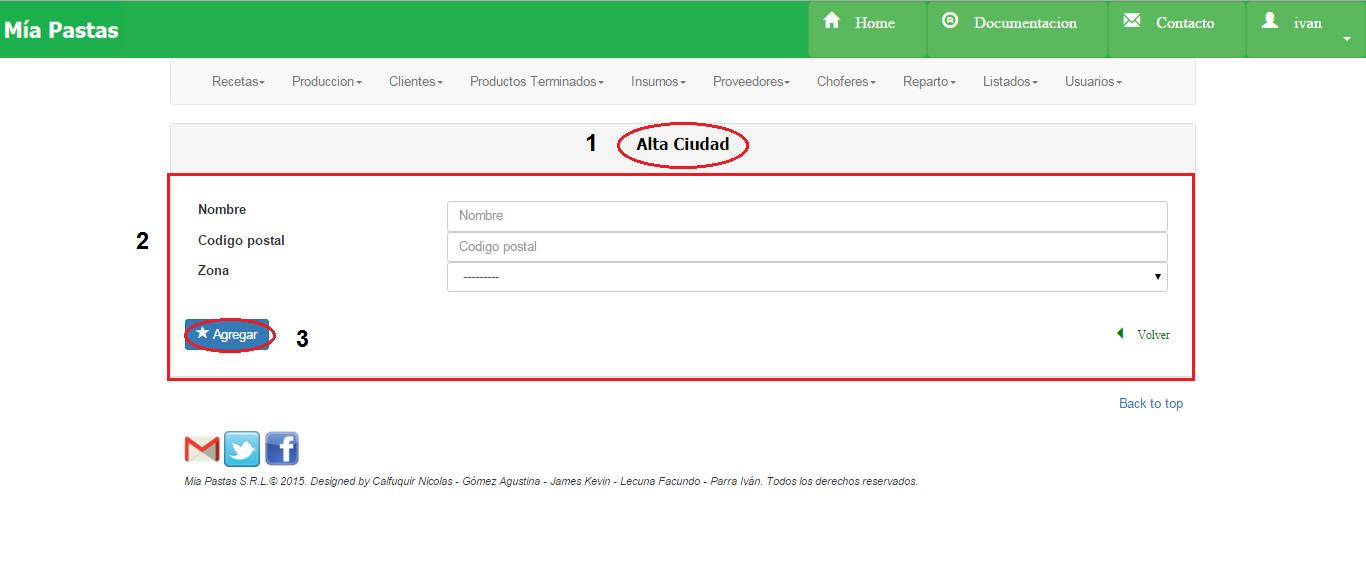
\includegraphics{ciudades_alta.jpg}
\begin{enumerate}
\item {} 
Nombre de la sección en la que nos ubicamos, (2) datos de la ciudad a crear, (3) confirmar el alta de nueva ciudad.

\end{enumerate}


\paragraph{{}Modificar Ciudades}
\label{ciudades modificar:modificar-ciudades}\label{ciudades modificar::doc}
Seleccionar con un click la ciudad a modificar, luego hacer click sobre el ícono de modificar.

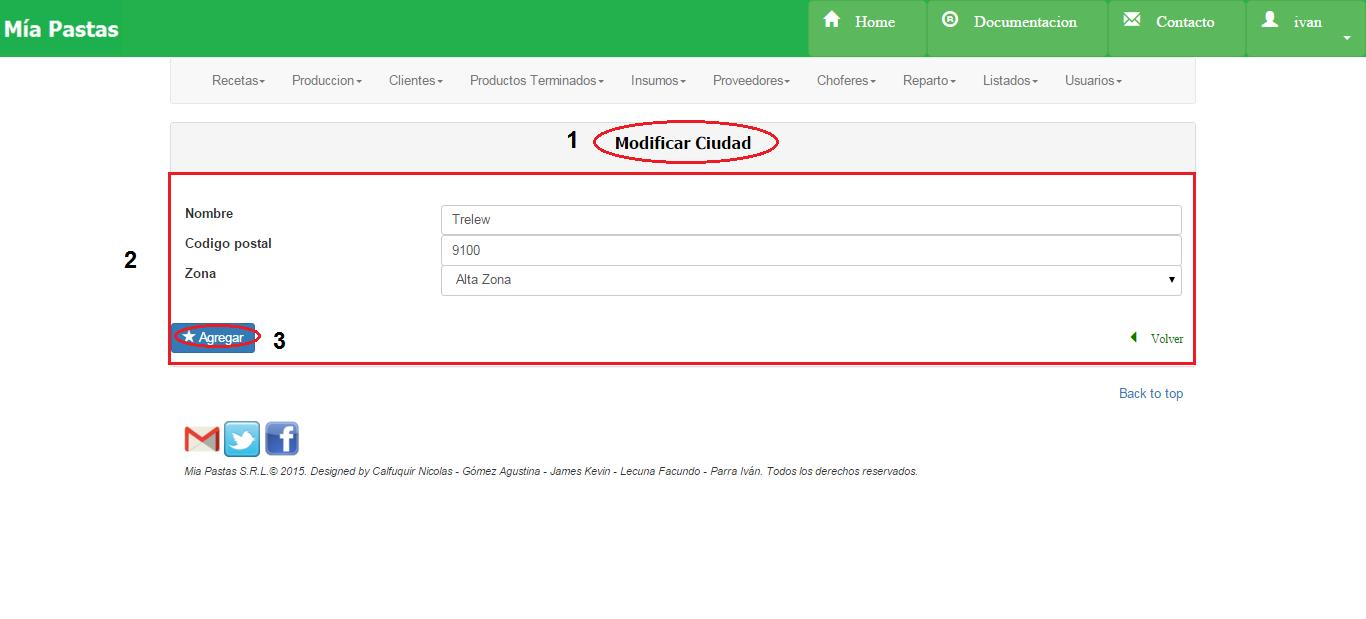
\includegraphics{ciudades_modificar.jpg}
\begin{enumerate}
\item {} 
Nombre de la sección en la que nos ubicamos, (2) descripción de la ciudad a modificar, (3)  guardar los cambios de la ciudad.

\end{enumerate}


\paragraph{{}Eliminar Ciudad}
\label{ciudades eliminar::doc}\label{ciudades eliminar:eliminar-ciudad}
Seleccionar con click una ciudad y hacer click sobre el botón de eliminar. Aparecerá el siguiente cartel:

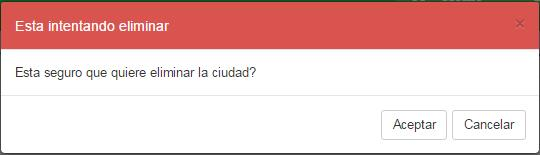
\includegraphics{ciudades_eliminar.jpg}

La ciudad no deberá tener clientes asociados


\subsection{{}Zonas}
\label{zonas:zonas}\label{zonas::doc}
En la pantalla de zonas podremos filtrar zonas por nombre, llenando la casilla nombre y presionando el botón filtrar.
Para poder filtrar todas las zonas el nombre deberá estar vacío y presionamos el botón filtrar.
.. image:: \_static/zonas/zonas\_ini.jpg


\subsubsection{{}Alta Zona}
\label{zonas alta:alta-zona}\label{zonas alta::doc}
Se deberá acceder al botón agregar desde la pantalla de zonas, luego se ingresará el nombre de la zona.
.. image:: \_static/zonas/zonas\_alta.jpg
Por el momento el detalle de las ciudades estará vacío por no contar con ciudades cargadas en la zona.
No se podrá cargar una zona que ya exista.


\subsection{{}Proveedores}
\label{proveedores:proveedores}\label{proveedores::doc}
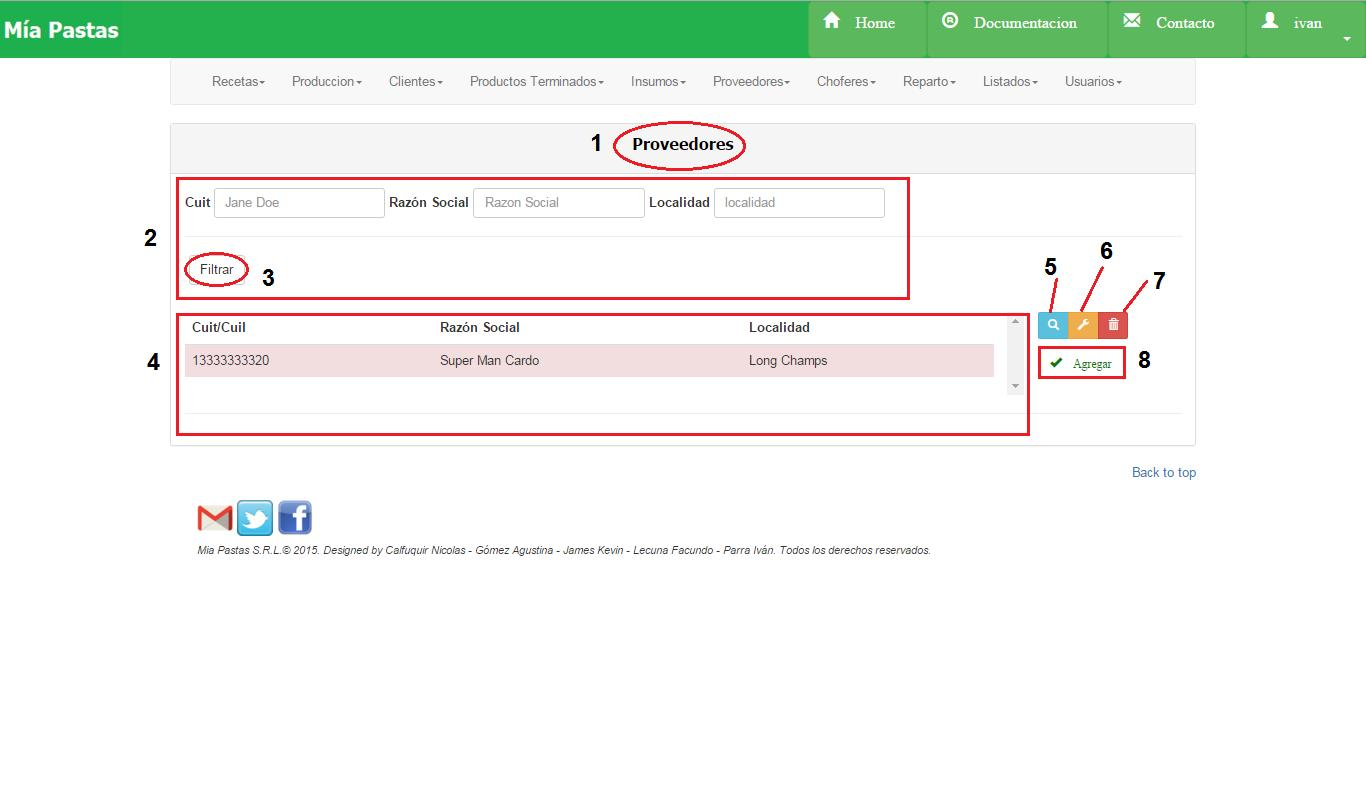
\includegraphics{proveedor_ini.jpg}
\begin{enumerate}
\item {} 
Nombre de la sección donde estamos ubicados.

\end{enumerate}

2.      Es el sector de filtrado, se podrá filtrar por cuit, razón social y/o localidad. Se filtrará presionando el botón (3).
4.      Área de resultado del filtro donde se mostrará el cuit, razón social y localidad de los proveedores filtrados. De no haberse realizado ningún filtro mostrará todos los insumos existentes.
5.      El icono de lupa sirve para mostrar más detalle sobre el ítem seleccionado como se muestra en la siguiente figura. De no seleccionar previamente un ítem aparecerá un mensaje de error.
6.      El icono de llave sirve para realizar una modificación sobre el ítem seleccionado. Para esto se deberá hacer click previamente sobre el ítem deseado. De no seleccionar previamente un ítem aparecerá un mensaje de error.


\subsubsection{Consultar Proveedores}
\label{proveedores:consultar-proveedores}
Seleccionar un proveedor haciendo click sobre el deseado y sobre el ícono de lupa.

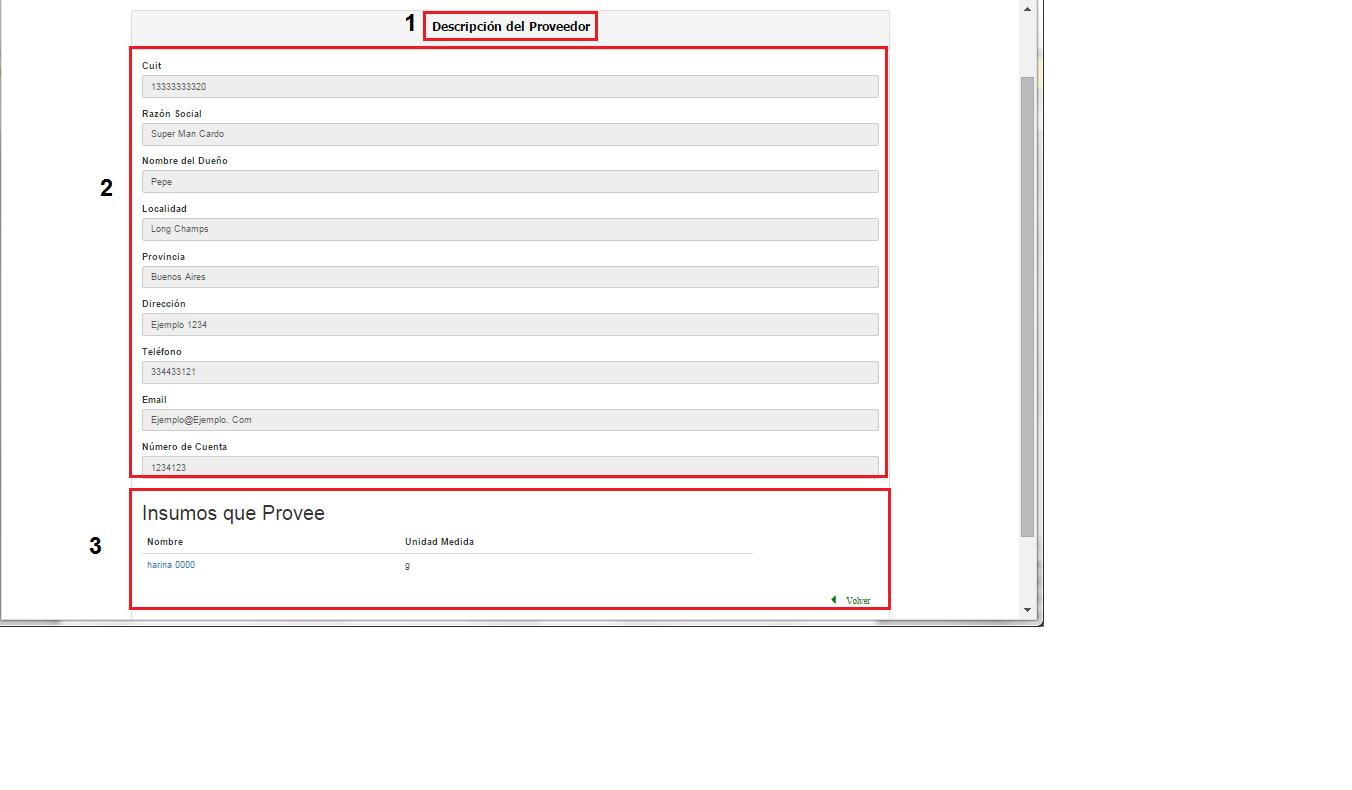
\includegraphics{proveedor_detalle.jpg}

En (1) vemos la sección en la que estamos ubicados, y en (2) vemos los datos del Proveedor seleccionado, mientras que en (3) vemos los insumos que provee ese proveedor.


\subsubsection{Modificar Proveedor}
\label{proveedores:modificar-proveedor}
Seleccionar con un click el proveedor a modificar, luego hacer click sobre el ícono de modificar.

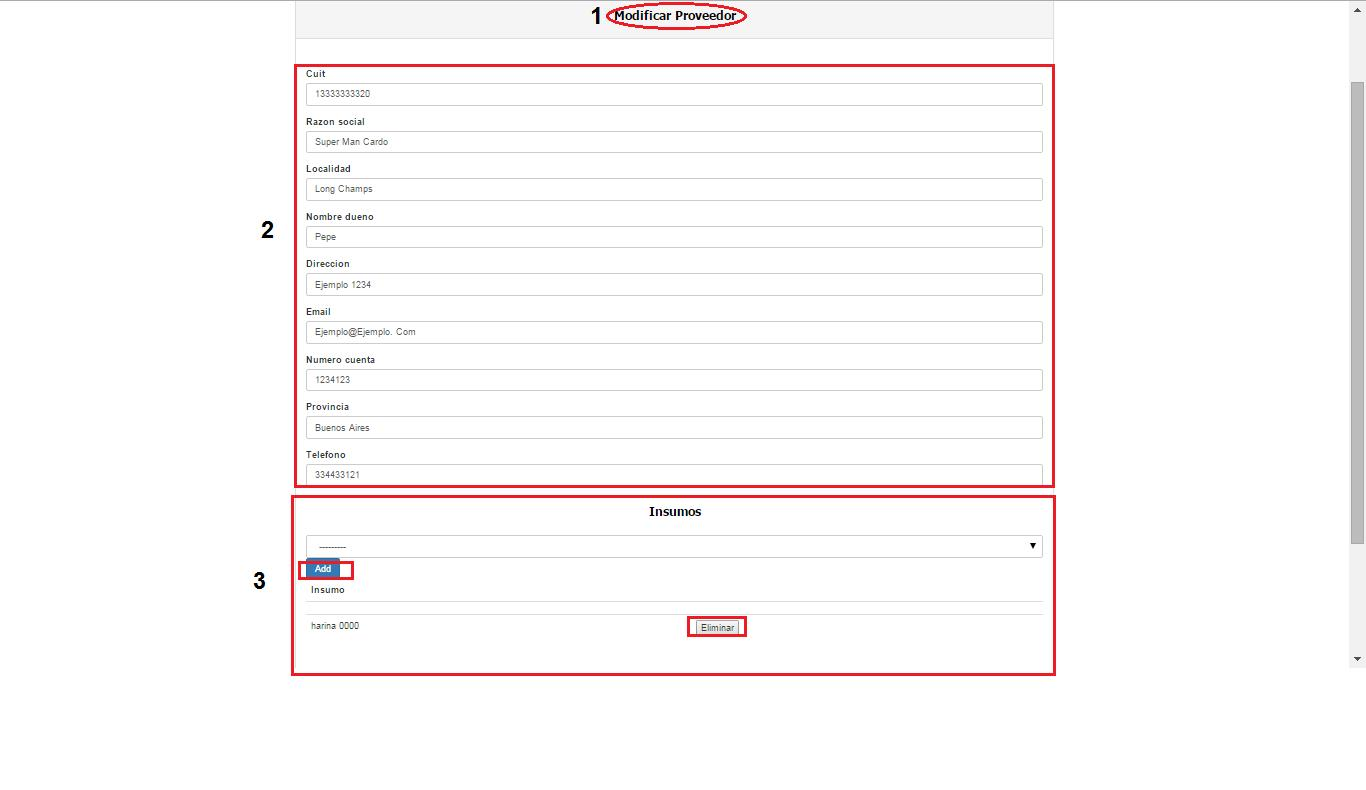
\includegraphics{proveedor_modificar.jpg}

En (1) vemos la sección donde estamos ubicados. La sección (2) y (3) se corresponde al área de modificación, será obligatorio completar que posean un asterisco (*).  En la sección (2) vemos los datos del proveedor, mientras que en (3) vemos los insumos provistos por ese proveedor, los cuales pueden ser modificados.


\subsubsection{Alta Proveedor}
\label{proveedores:alta-proveedor}
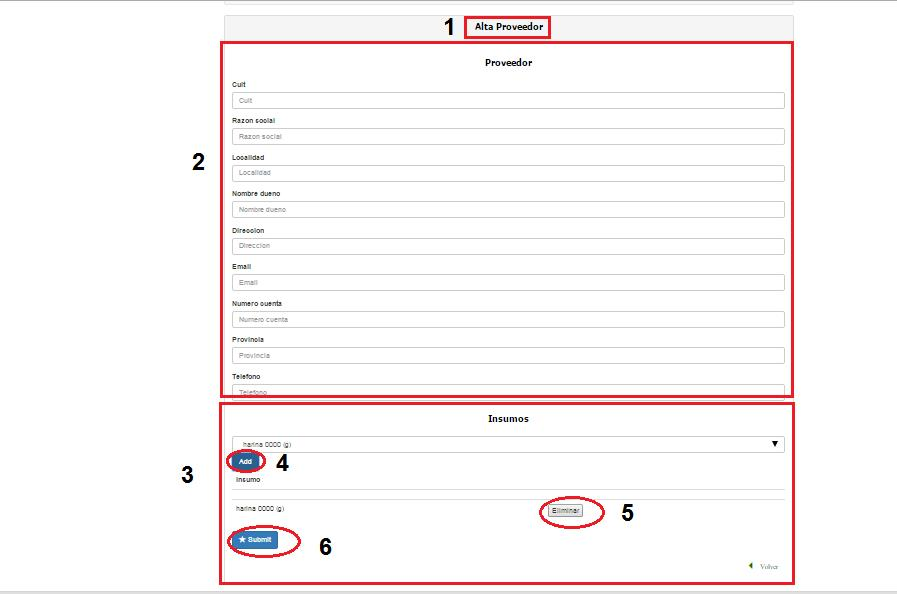
\includegraphics{proveedor_alta.jpg}

(1) Nombre de la sección en la que nos ubicamos, (2) datos a completar del proveedor a crear, (3) datos a completar de los insumos que provee ese proveedor, donde:
•       (4) permite agregar un insumo.
•       (5) permite eliminar un insumo del proveedor.
•       (6) permite dar de alta al nuevo proveedor.


\subsubsection{Eliminar Proveedores}
\label{proveedores:eliminar-proveedores}
Seleccionar con click un proveedor y hacer click sobre el botón de eliminar. Aparecerá el siguiente cartel:

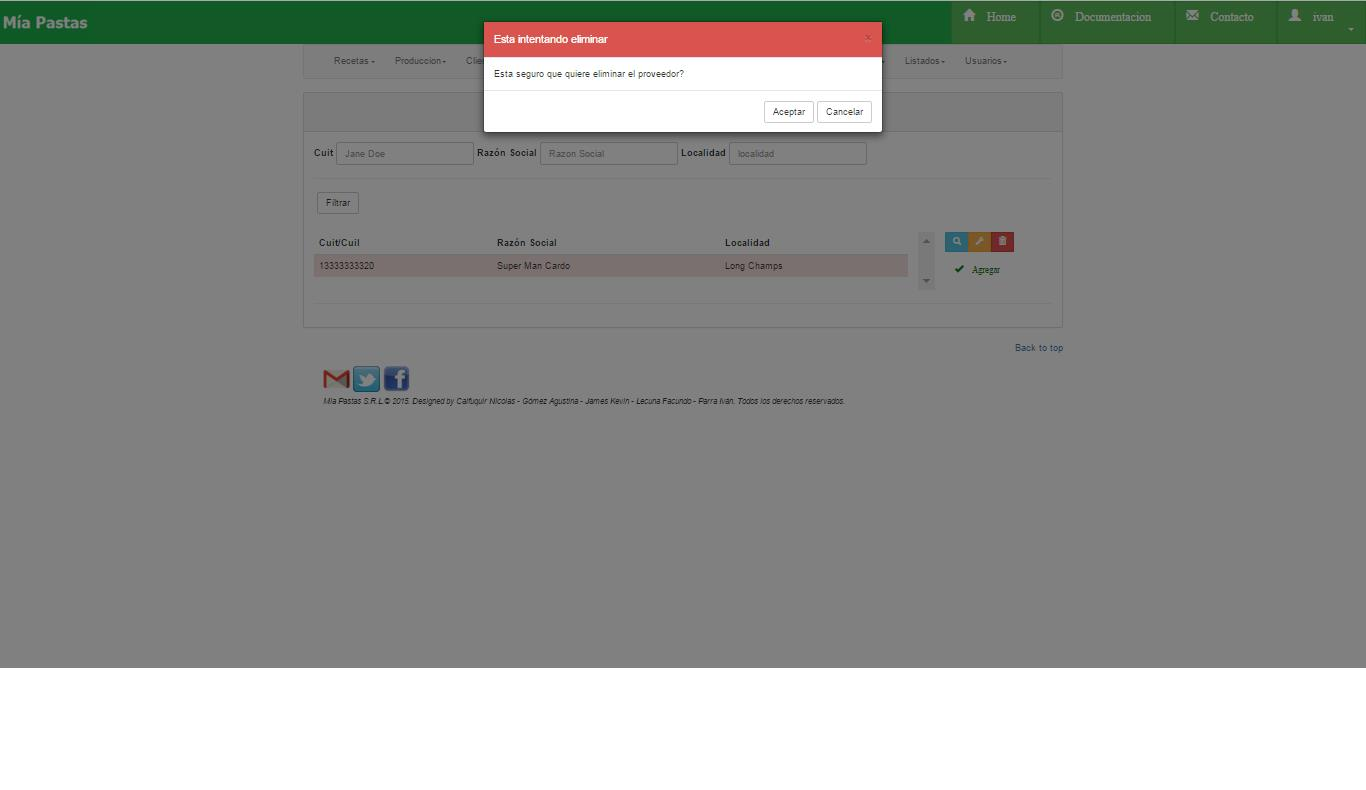
\includegraphics{proveedor_eliminar.jpg}

El proveedor no deberá tener pedidos asociados


\paragraph{{}Consultar Proveedores}
\label{proveedores consultarConsult:consultar-proveedores}\label{proveedores consultarConsult::doc}
Seleccionar un proveedor haciendo click sobre el deseado y sobre el ícono de lupa.

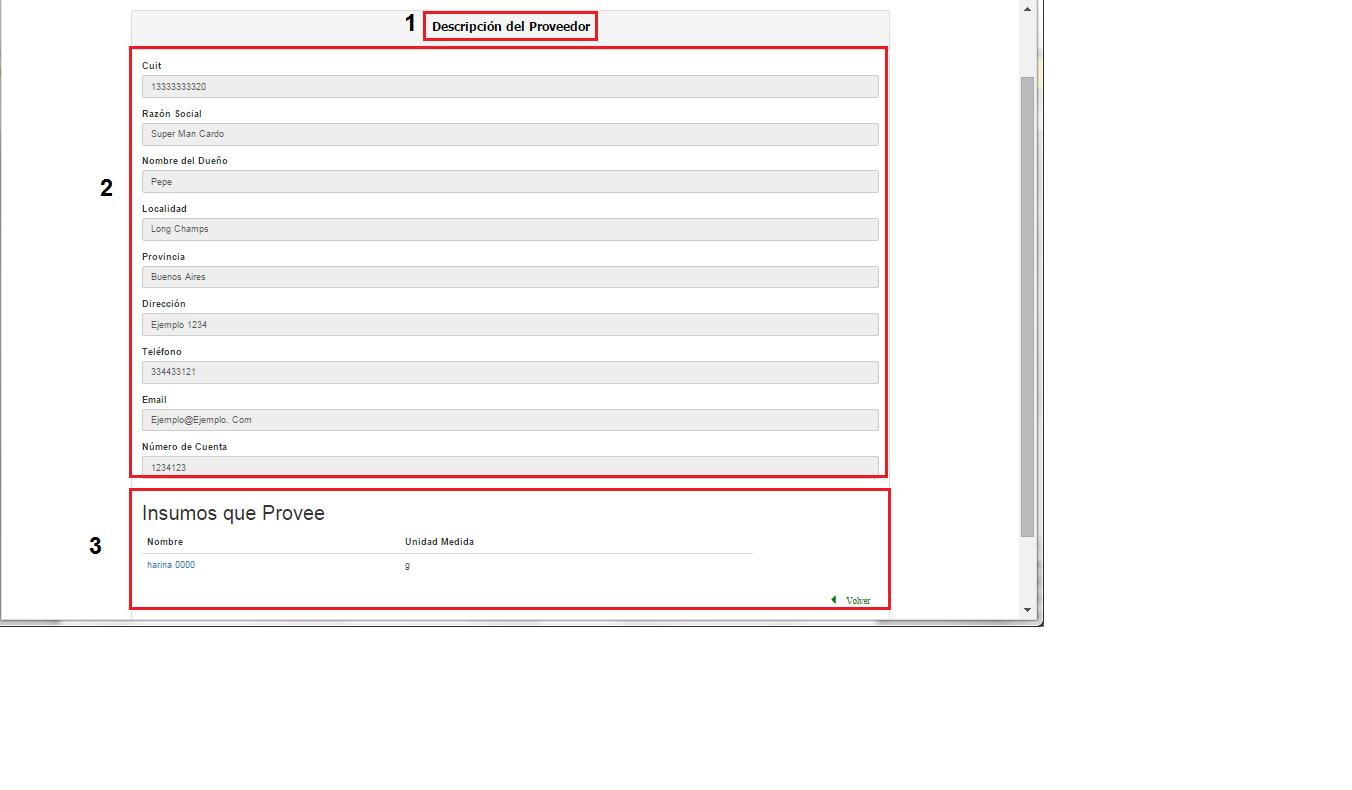
\includegraphics{proveedor_detalle.jpg}

En (1) vemos la sección en la que estamos ubicados, y en (2) vemos los datos del Proveedor seleccionado, mientras que en (3) vemos los insumos que provee ese proveedor.


\paragraph{{}Alta Proveedor}
\label{proveedores Alta:alta-proveedor}\label{proveedores Alta::doc}
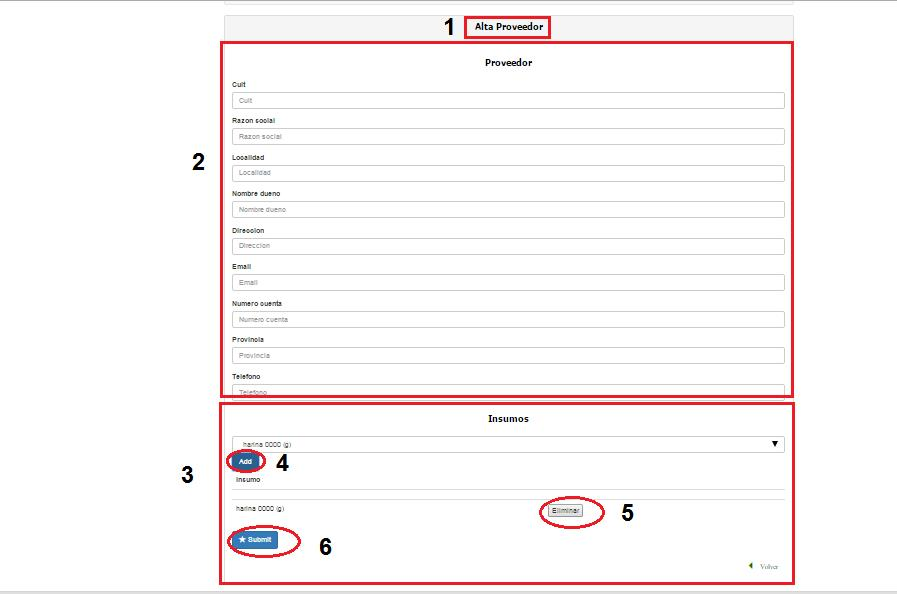
\includegraphics{proveedor_alta.jpg}

(1) Nombre de la sección en la que nos ubicamos, (2) datos a completar del proveedor a crear, (3) datos a completar de los insumos que provee ese proveedor, donde:
•       (4) permite agregar un insumo.
•       (5) permite eliminar un insumo del proveedor.
•       (6) permite dar de alta al nuevo proveedor.


\paragraph{{}Modificar Proveedor}
\label{proveedores consultarModifica:modificar-proveedor}\label{proveedores consultarModifica::doc}
Seleccionar con un click el proveedor a modificar, luego hacer click sobre el ícono de modificar.

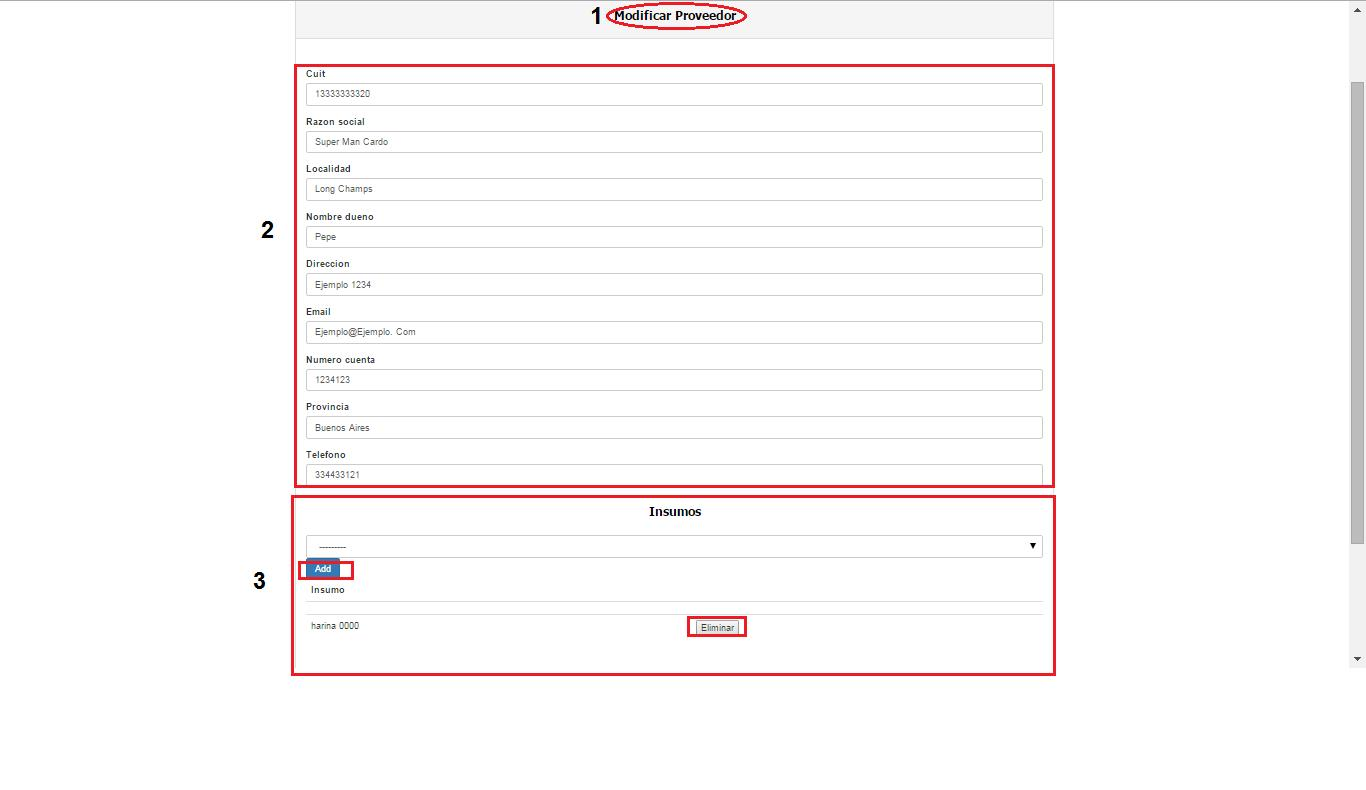
\includegraphics{proveedor_modificar.jpg}

En (1) vemos la sección donde estamos ubicados. La sección (2) y (3) se corresponde al área de modificación, será obligatorio completar que posean un asterisco (*).  En la sección (2) vemos los datos del proveedor, mientras que en (3) vemos los insumos provistos por ese proveedor, los cuales pueden ser modificados.


\paragraph{{}Eliminar Proveedores}
\label{proveedores eliminar:eliminar-proveedores}\label{proveedores eliminar::doc}
Seleccionar con click un proveedor y hacer click sobre el botón de eliminar. Aparecerá el siguiente cartel:

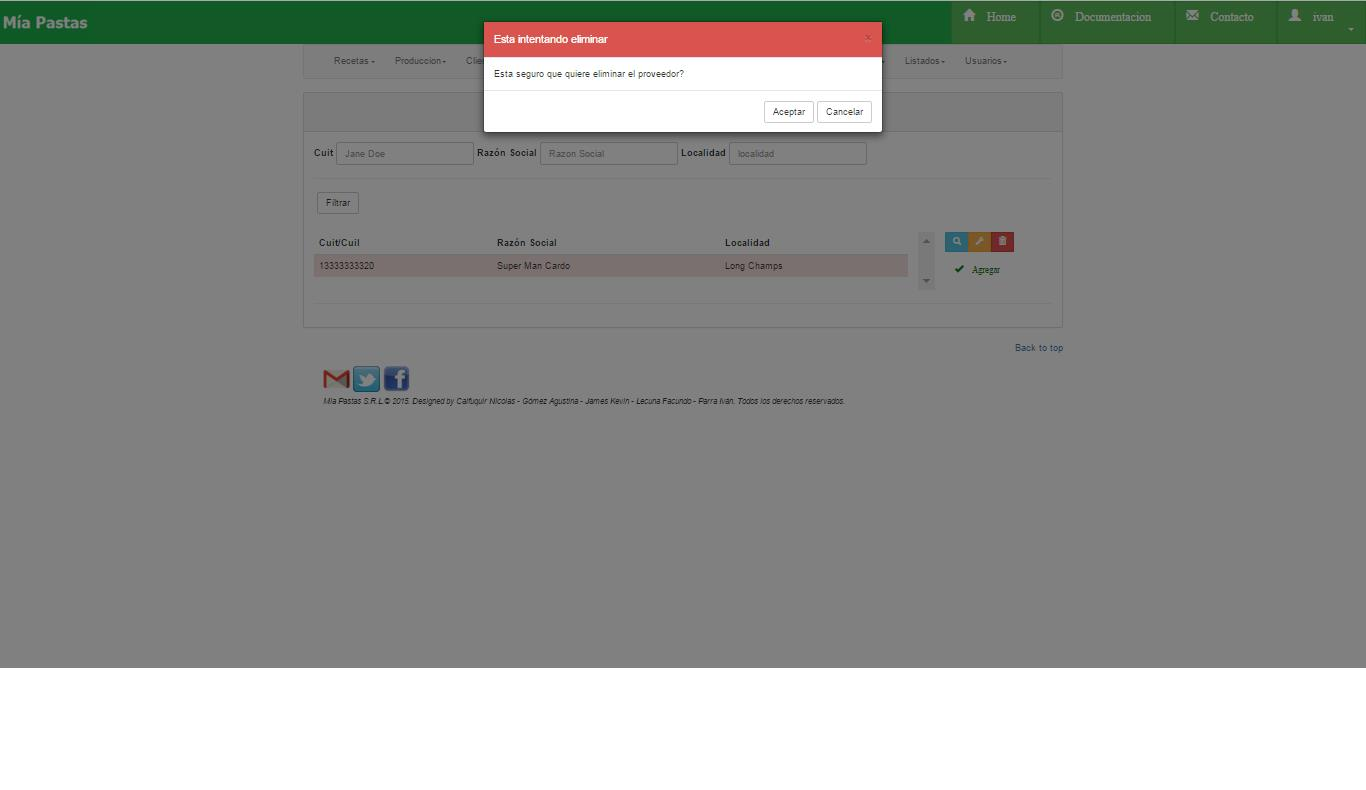
\includegraphics{proveedor_eliminar.jpg}

El proveedor no deberá tener pedidos asociados


\subsection{{}Proveedores}
\label{pedidosProveedor:proveedores}\label{pedidosProveedor::doc}
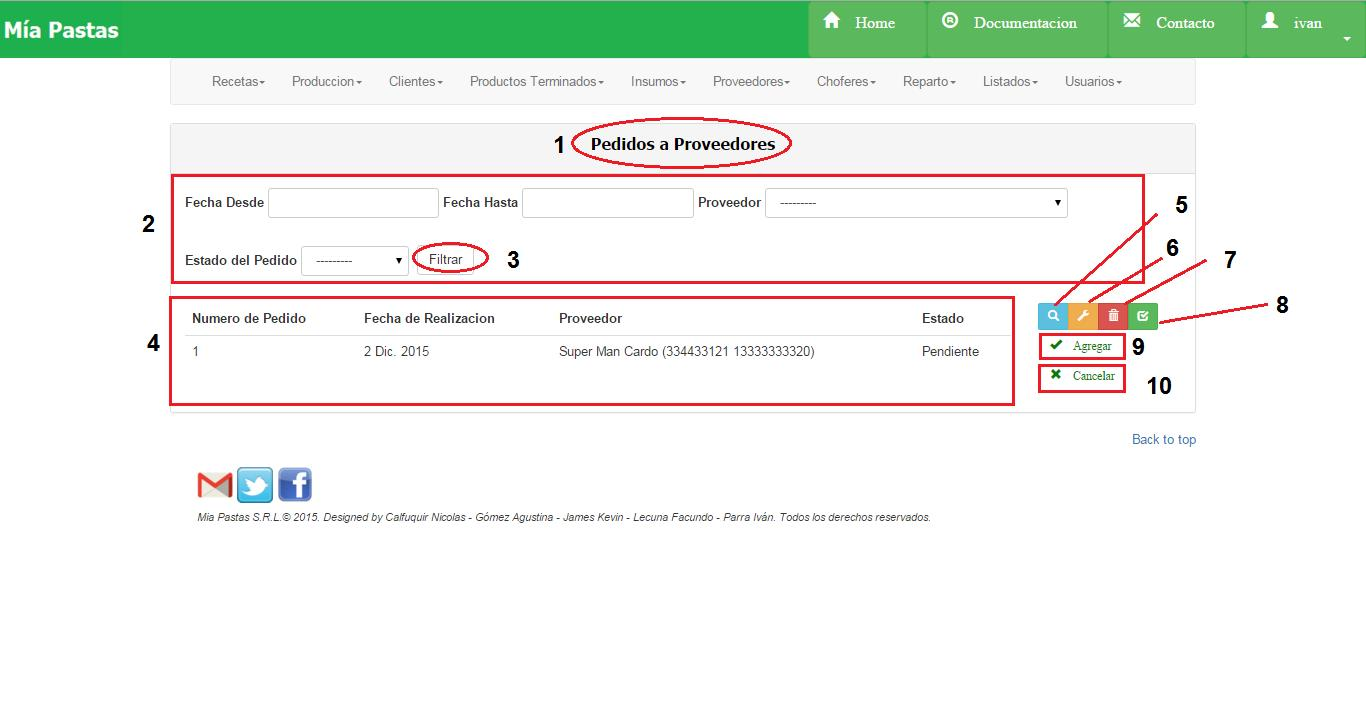
\includegraphics{pedidos_ini.jpg}
\begin{enumerate}
\item {} 
Nombre de la sección donde estamos ubicados.

\end{enumerate}

2.      Es el sector de filtrado, se podrá filtrar por fecha desde, fecha hasta, proveedor y/o estado del pedido. Se filtrará presionando el botón (3).
4.      Área de resultado del filtro donde se mostrará número de pedido, fecha de realización, proveedor y estado de los pedidos a proveedor filtrados. De no haberse realizado ningún filtro mostrará todos los proveedores existentes.
5.      El icono de lupa sirve para mostrar más detalle sobre el ítem seleccionado. De no seleccionar previamente un ítem aparecerá un mensaje de error.
6.      El icono de llave sirve para realizar una modificación sobre el ítem seleccionado. Para esto se deberá hacer click previamente sobre el ítem deseado. De no seleccionar previamente un ítem aparecerá un mensaje de error.
7.      El icono del tacho de basura (2) sirve para eliminar un elemento seleccionado. Para esto se deberá hacer click previamente sobre el ítem que se desea eliminar (1). De no seleccionar previamente un ítem aparecerá un mensaje de error.
8.      El icono del tilde (8) sirve para recepcionar un pedido seleccionado. Para esto se deberá hacer click previamente sobre el pedido que se desea recepcionar. De no seleccionar previamente un pedido aparecerá un mensaje de error.
9.      Este botón permite abrir el formulario para dar de Alta un Nuevo Proveedor.
10.     Este botón permite Cancelar el Pedido realizado a un proveedor. Para ello, debemos seleccionar el pedido y luego presionar el botón.


\subsubsection{Consultar Pedido a Proveedores}
\label{pedidosProveedor:consultar-pedido-a-proveedores}
Seleccionar un pedido a proveedor haciendo click sobre el deseado y sobre el ícono de lupa.

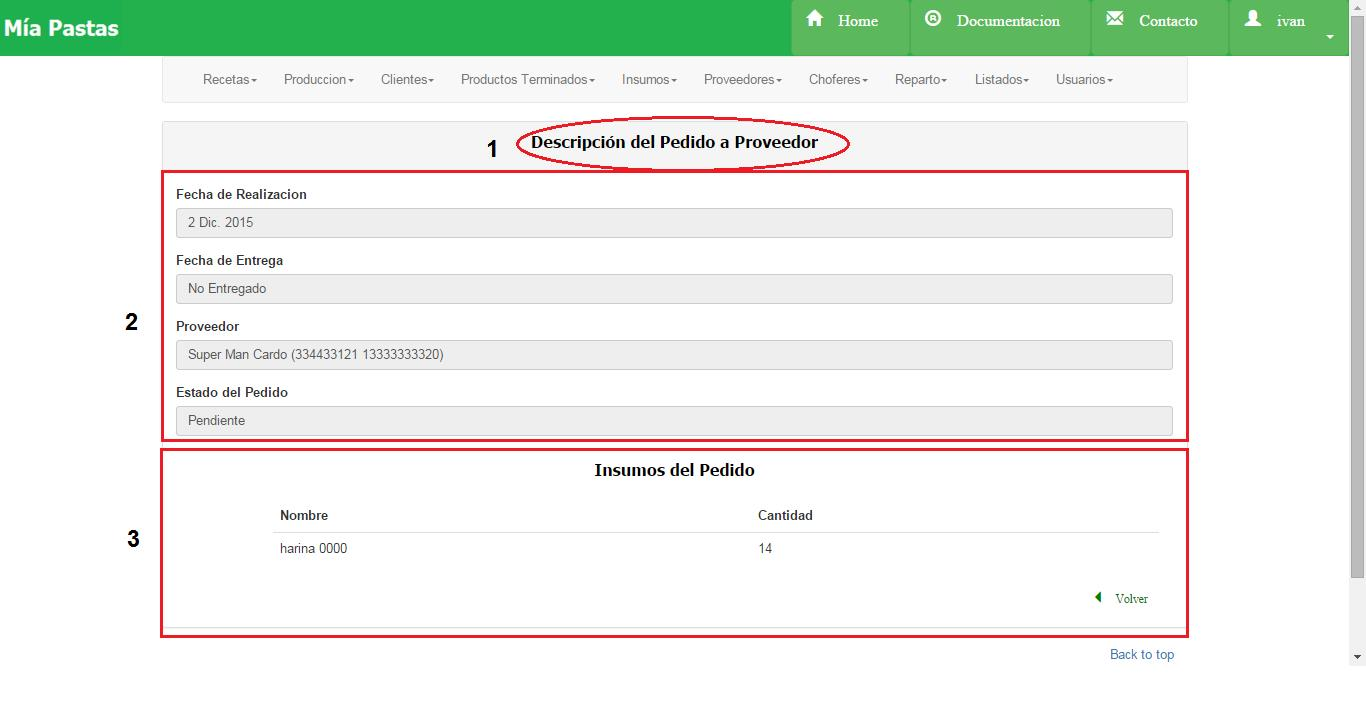
\includegraphics{pedidos_detalle.jpg}

En (1) vemos la sección en la que estamos ubicados, en (2) vemos los datos del pedido seleccionado, y en (3) vemos el detalle del pedido, es decir, los insumos y cantidad pedidos.


\subsubsection{Modificar Pedido a Proveedor}
\label{pedidosProveedor:modificar-pedido-a-proveedor}
Seleccionar con un click el pedido a proveedor a modificar, luego hacer click sobre el ícono de modificar.

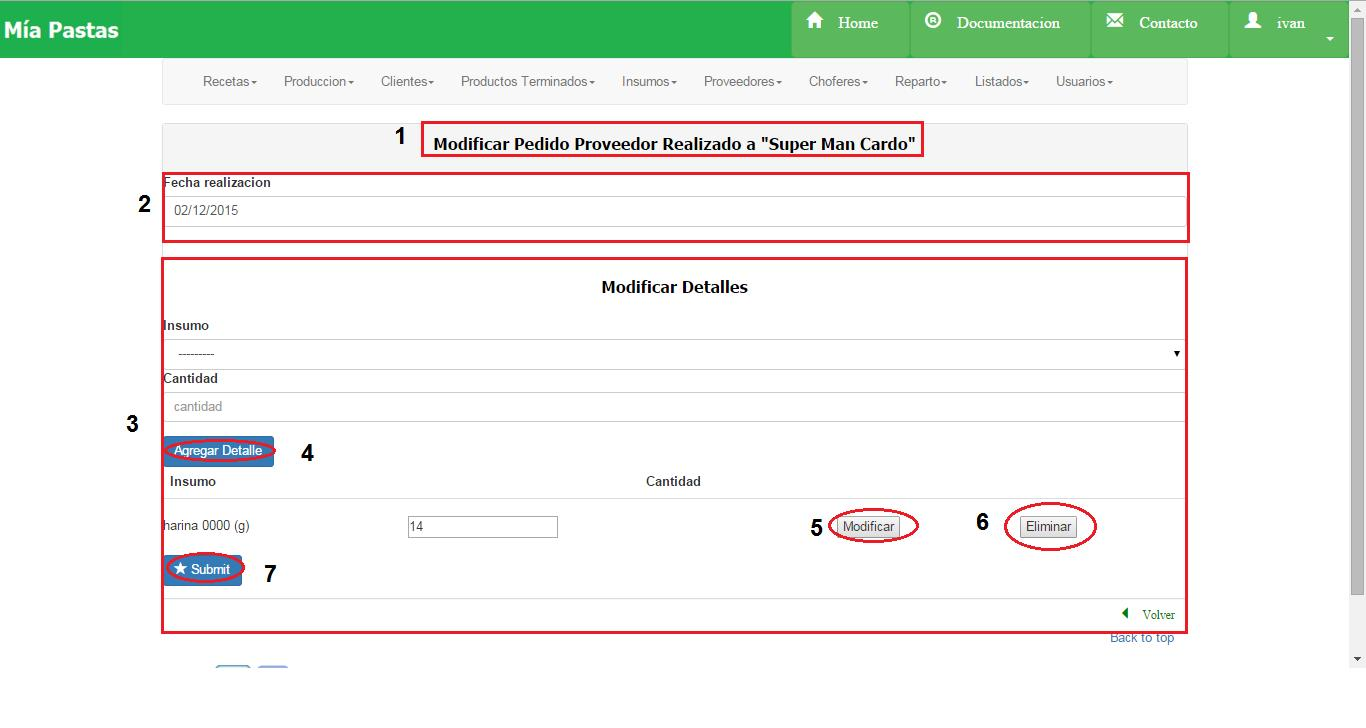
\includegraphics{pedidos_modificar.jpg}

En (1) vemos la sección donde estamos ubicados. La sección (2) y (3) se corresponden al área de modificación, será obligatorio completar los campos que posean un asterisco (*). En la sección (2) podremos modificar la fecha de realización del pedido. En (3) podremos modificar el detalle del pedido, es decir, los insumos y cantidades solicitados. El botón (43) permite agregar un insumo como comercializado por el proveedor, mientras que el (6) permite eliminarlo. El botón (5) permite modificar la cantidad solicitada del insumo. El botón (7) permite guardar los cambios realizados.


\subsubsection{Recepcionar Pedido a Proveedor}
\label{pedidosProveedor:recepcionar-pedido-a-proveedor}
Seleccionar con un click el pedido a proveedor a recepcionar, luego hacer click sobre el ícono de recepcionar.

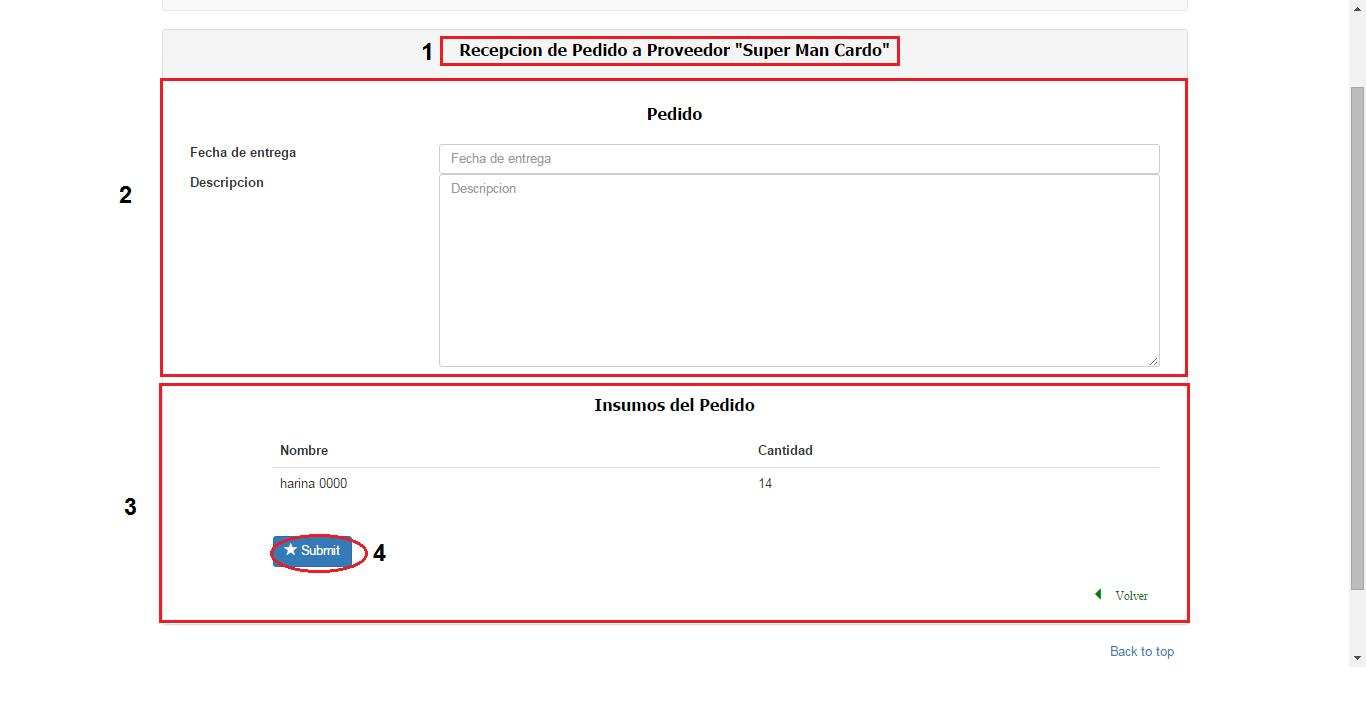
\includegraphics{pedidos_recepcionar.jpg}

En (1) vemos la sección donde estamos ubicados. La sección (2) y (3) se corresponde al área de recepción, será obligatorio completar que posean un asterisco (*).  En la sección (2) debemos ingresar la fecha de entrega y descripción del pedido, mientras que en (3) vemos los insumos que hemos pedido a ese proveedor. Al presionar el botón (4) se recepcionará el pedido, pasando al estado “Recibido” y actualizando el stock automáticamente de cada insumo.


\subsubsection{Alta Pedido a Proveedor}
\label{pedidosProveedor:alta-pedido-a-proveedor}
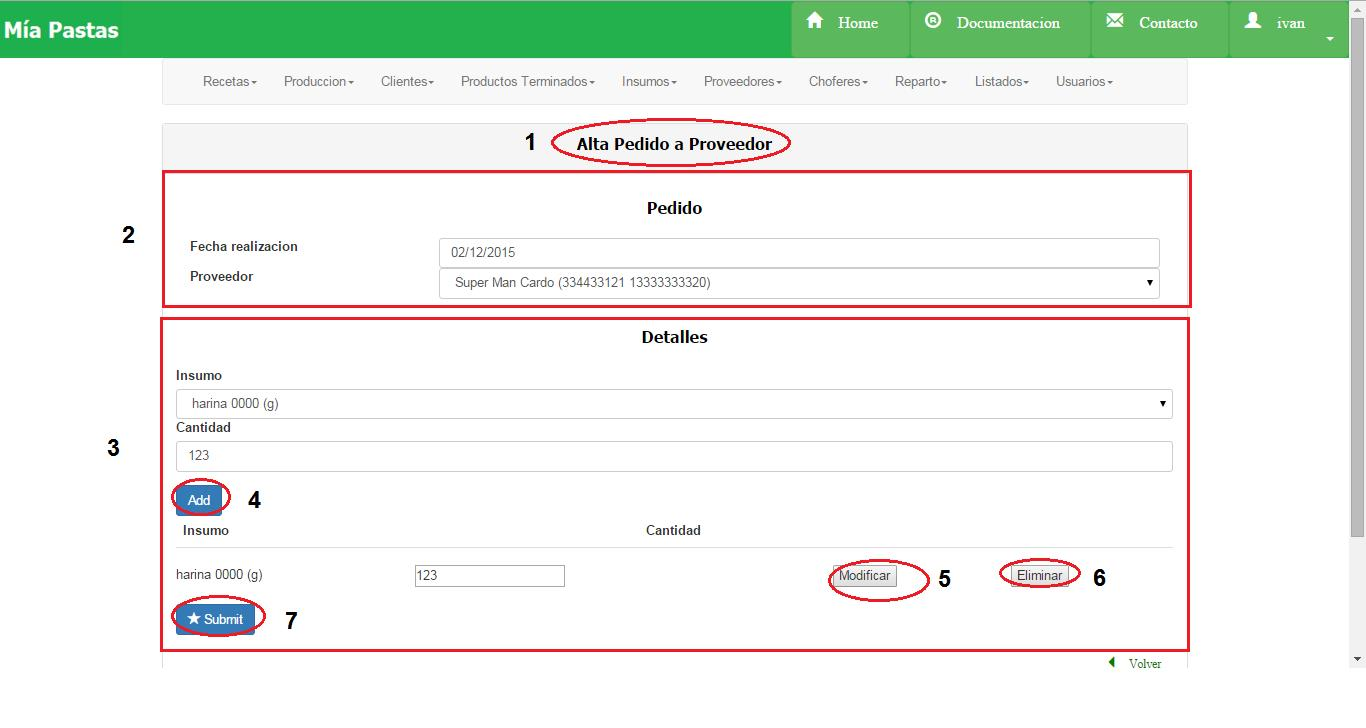
\includegraphics{pedidos_alta.jpg}

(1) Nombre de la sección en la que nos ubicamos, (2) datos a completar del insumo a crear, (3) datos a completar de los insumos y cantidades del pedido, donde:
•       (4) permite agregar un insumo.
•       (5) permite modificar la cantidad de un insumo.
•       (6) permite eliminar un insumo del pedido.
•       (7) permite dar de alta al nuevo proveedor.


\subsubsection{Eliminar Pedido a Proveedores}
\label{pedidosProveedor:eliminar-pedido-a-proveedores}
Seleccionar con click un pedido a proveedor y hacer click sobre el botón de eliminar. Aparecerá el siguiente cartel:

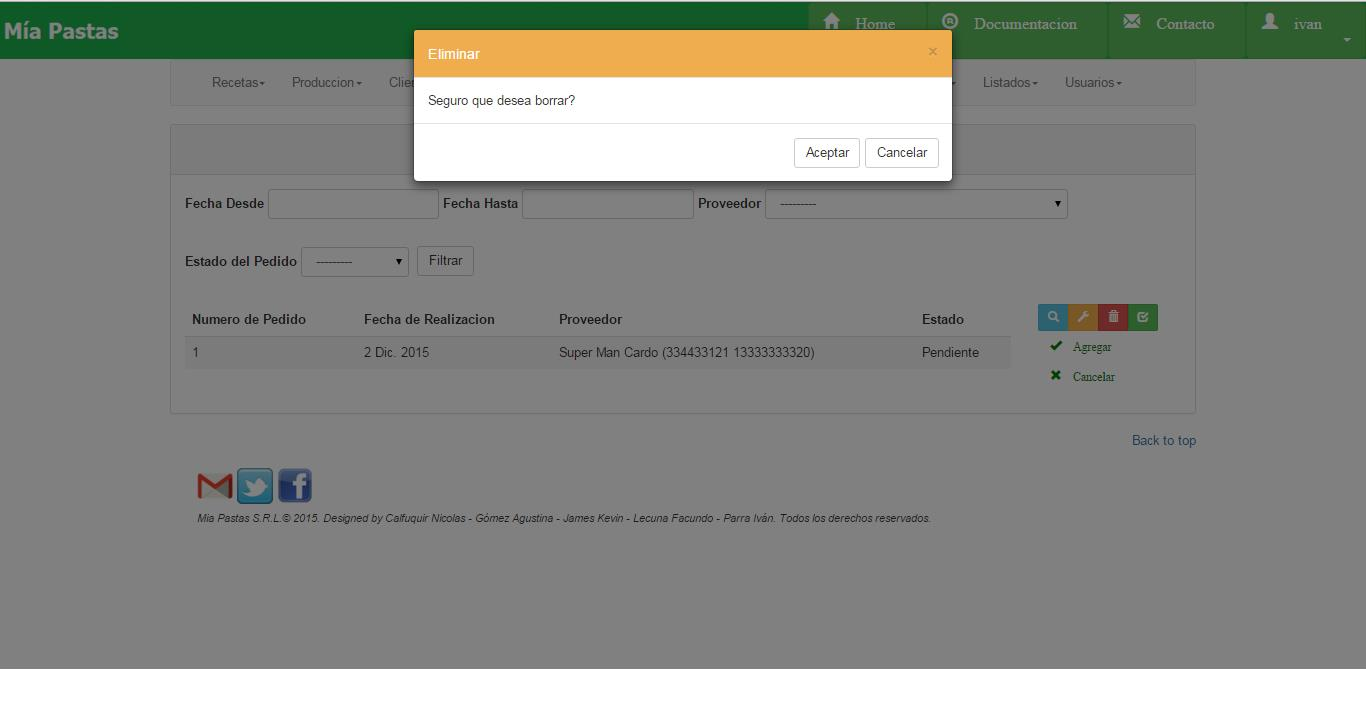
\includegraphics{pedidos_eliminar.jpg}


\paragraph{{}Recepcionar pedidos a Proveedor}
\label{pedidosProveedor consultarrecepciona::doc}\label{pedidosProveedor consultarrecepciona:recepcionar-pedidos-a-proveedor}
Seleccionar con un click el pedido a proveedor a recepcionar, luego hacer click sobre el ícono de recepcionar.

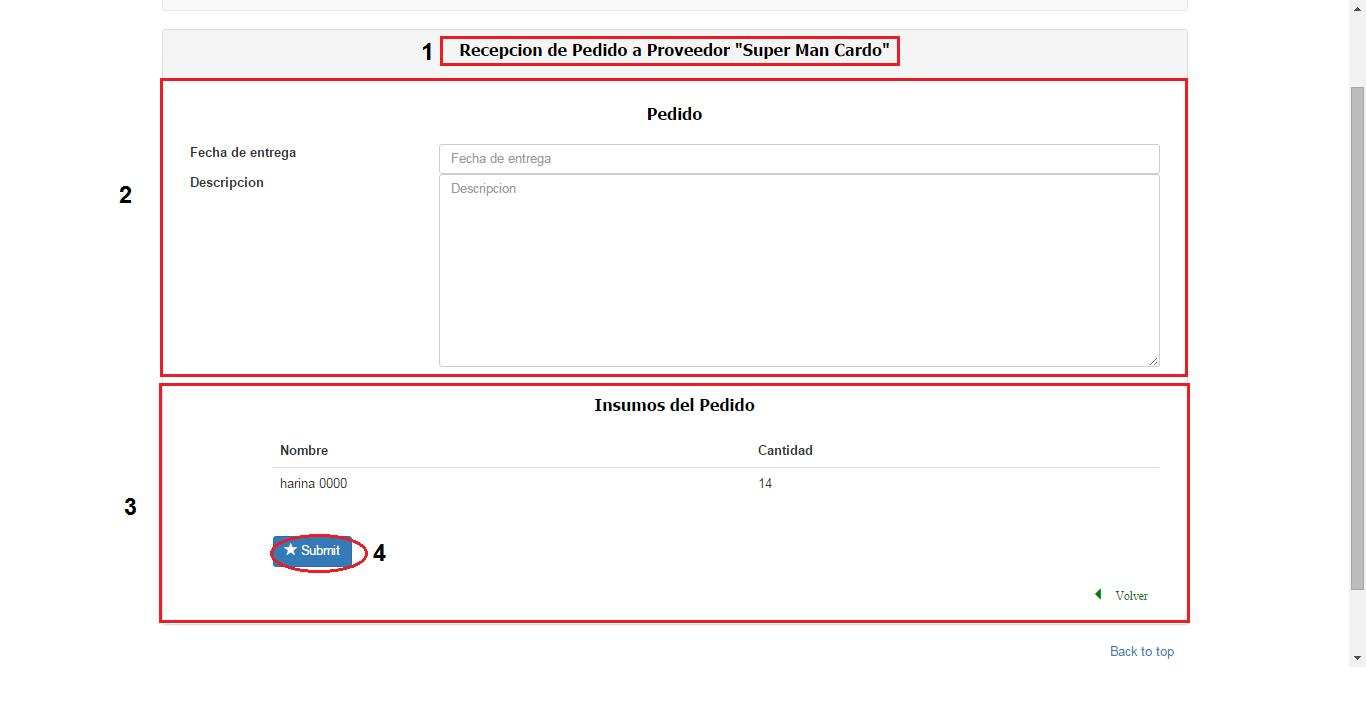
\includegraphics{pedidos_recepcionar.jpg}

En (1) vemos la sección donde estamos ubicados. La sección (2) y (3) se corresponde al área de recepción, será obligatorio completar que posean un asterisco (*).  En la sección (2) debemos ingresar la fecha de entrega y descripción del pedido, mientras que en (3) vemos los insumos que hemos pedido a ese proveedor. Al presionar el botón (4) se recepcionará el pedido, pasando al estado “Recibido” y actualizando el stock automáticamente de cada insumo.


\subsection{{}Choferes}
\label{choferes::doc}\label{choferes:choferes}
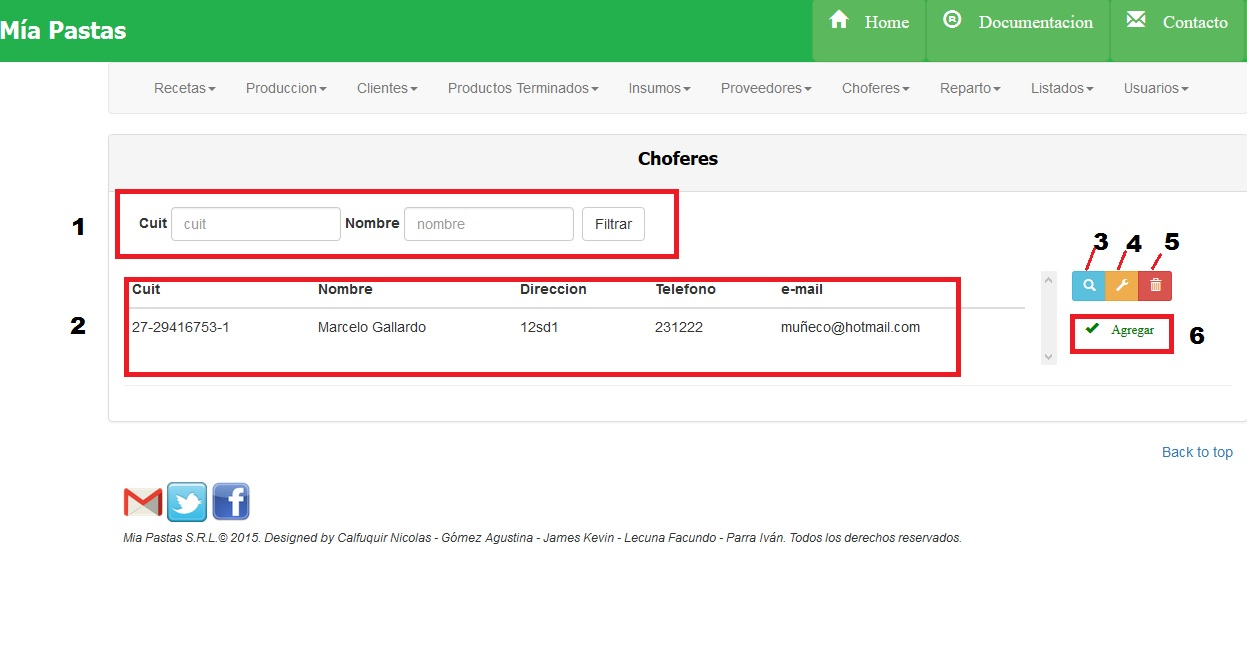
\includegraphics{chofer_inicio.jpg}
\begin{enumerate}
\item {} 
Es el sector de filtrado, se podrá filtrar por cuit o por nombre del chofer.

\item {} 
Área de resultado del filtro donde se mostrará cuit, nombre, dirección, teléfono y e-mail, de no haberse realizado ningún filtro mostrará todos los choferes.

\item {} 
El icono de lupa sirve para mostrar más detalle sobre el ítem seleccionado como se muestra en la siguiente figura (1), para volver a la pantalla anterior se deberá hacer click sobre volver (2). De no seleccionar previamente un ítem aparecerá un mensaje de error.

\item {} 
El icono de llave sirve para realizar una modificación sobre el ítem seleccionado. Para esto se deberá hacer click previamente sobre el chofer deseado. De no seleccionar previamente un ítem aparecerá un mensaje de error.

\item {} 
El icono del tacho de basura (2) sirve para eliminar un elemento seleccionado. Para esto se deberá hacer click previamente sobre el ítem que se desea eliminar (1). De no seleccionar previamente un ítem aparecerá un mensaje de error.

\end{enumerate}


\subsubsection{Consultar Choferes}
\label{choferes:consultar-choferes}
Seleccionar un chofer haciendo click sobre el deseado y sobre el ícono de lupa.

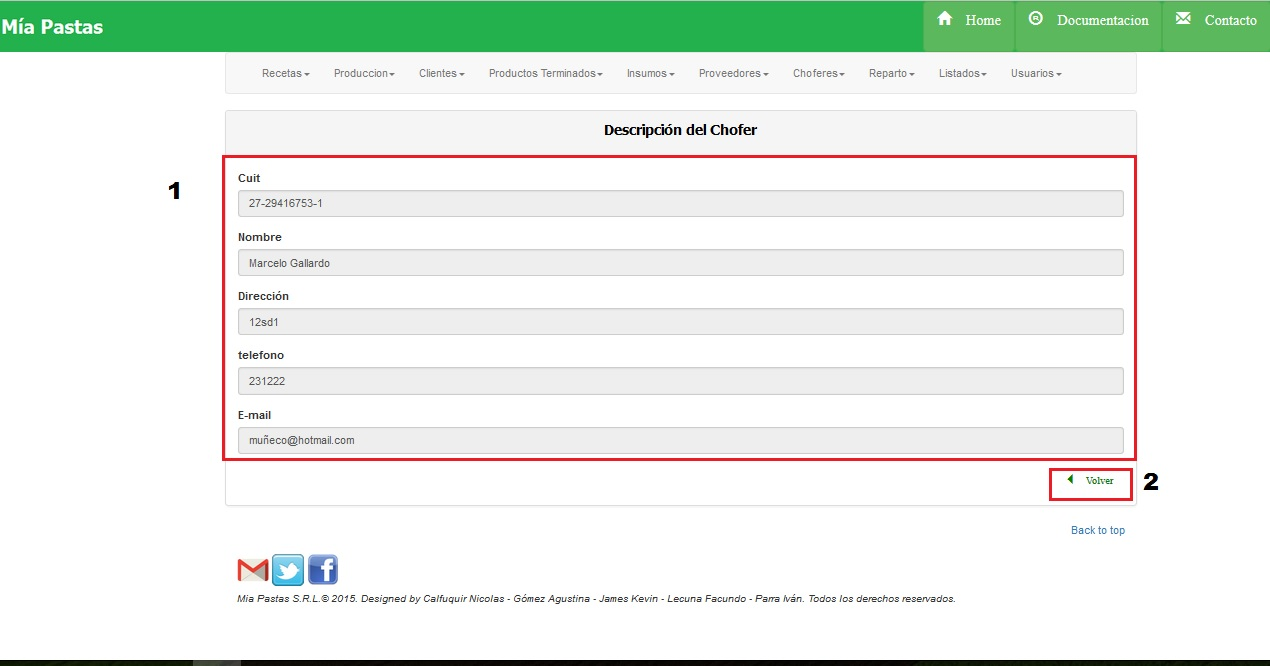
\includegraphics{chofer_detalle.jpg}
\begin{enumerate}
\item {} 
Nombre de la sección en la que nos ubicamos, (2) descripción del chofer consultado.

\end{enumerate}


\subsubsection{Modificar Chofer}
\label{choferes:modificar-chofer}
Seleccionar con un click el chofer a modificar, luego hacer click sobre el ícono de modificar.

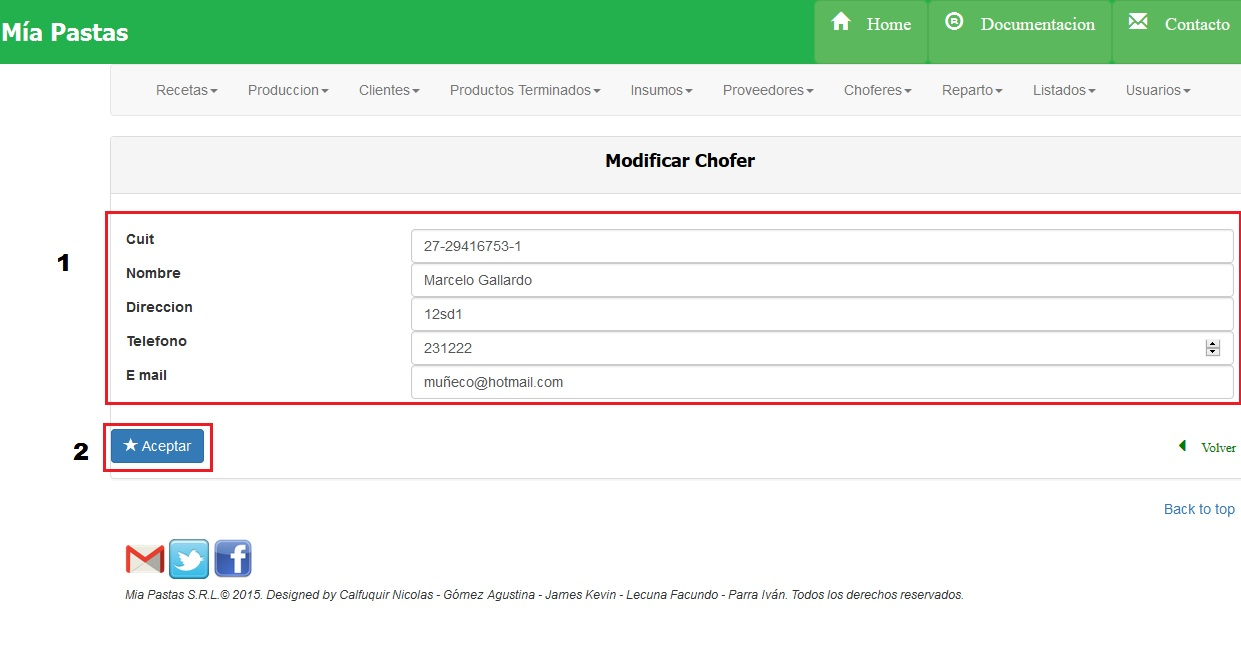
\includegraphics{chofer_modificar.jpg}

La sección (1) se corresponde al área de modificación, será obligatorio completar los campos nombre y cuit. En la sección (2) se encuentra el botón de aceptar para guardar los cambios.


\subsubsection{Alta Chofer}
\label{choferes:alta-chofer}
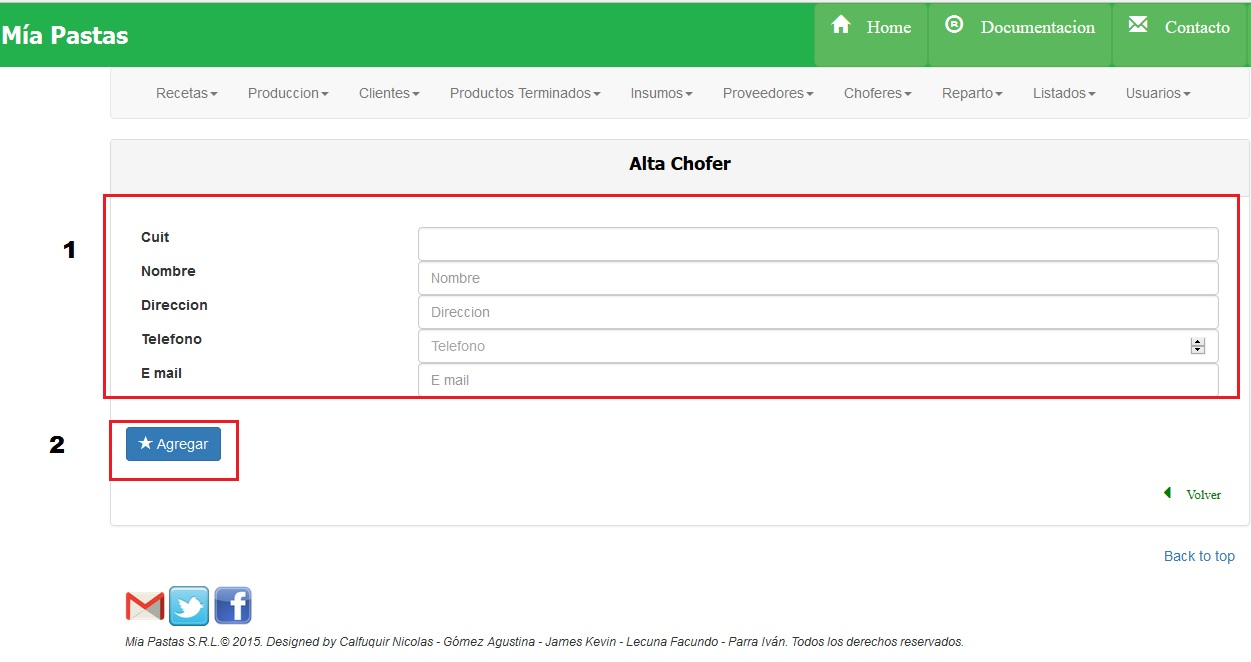
\includegraphics{chofer_alta.jpg}
\begin{enumerate}
\item {} 
Nombre de la sección en la que nos ubicamos, (2) datos del chofer a crear, (3) confirmar alta nuevo chofer.

\end{enumerate}


\subsubsection{Eliminar Choferes}
\label{choferes:eliminar-choferes}
Seleccionar con click un chofer y hacer click sobre el botón de eliminar. Aparecerá el siguiente cartel:

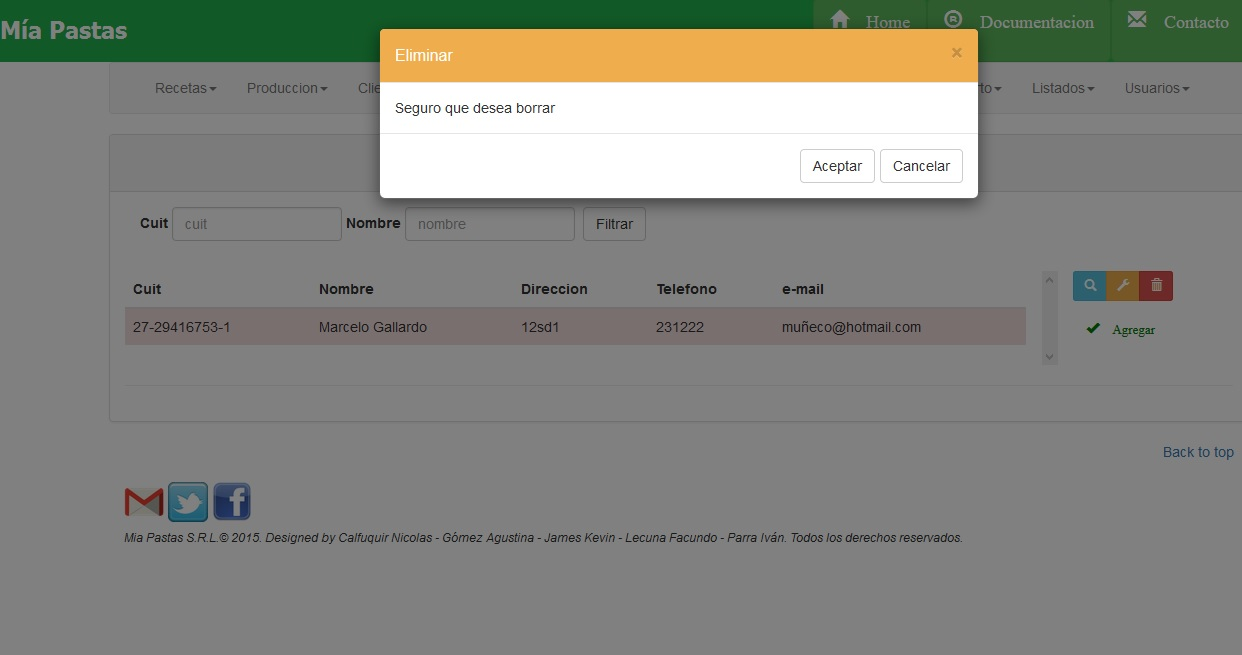
\includegraphics{chofer_eliminar.jpg}

El chofer no deberá tener hojas de ruta vigentes asociadas


\paragraph{{}Consultar Choferes}
\label{choferes consultar:consultar-choferes}\label{choferes consultar::doc}
Seleccionar un chofer haciendo click sobre el deseado y luego haciendo click sobre el ícono de lupa

\includegraphics{chofer_detalle.jpg}
\begin{enumerate}
\item {} 
Nombre de la sección en la que nos ubicamos, (2) descripción del chofer consultado.

\end{enumerate}


\paragraph{{}Alta Chofer}
\label{choferes alta:alta-chofer}\label{choferes alta::doc}
\includegraphics{chofer_alta.jpg}
\begin{enumerate}
\item {} 
Nombre de la sección en la que nos ubicamos, (2) datos del chofer a crear, (3) confirmar alta nuevo chofer.

\end{enumerate}


\paragraph{{}Modificar Ciudad}
\label{choferes modificar:modificar-ciudad}\label{choferes modificar::doc}
Seleccionar con un click la ciudad a modificar, luego hacer click sobre el ícono de modificar.

\includegraphics{_static/ciudades/ciudad_modificar.jpg}
\begin{enumerate}
\item {} 
Nombre de la sección en la que nos ubicamos, (2) descripción de la ciudad a modificar, (3)  guardar los cambios de la ciudad.

\end{enumerate}


\paragraph{{}Eliminar Choferes}
\label{choferes eliminar:eliminar-choferes}\label{choferes eliminar::doc}
Seleccionar con click un chofer y hacer click sobre el botón sobre el ícono de eliminar. Aparecerá el siguiente cartel:

\includegraphics{chofer_eliminar.jpg}

El chofer no deberá tener hojas de ruta vigentes asociadas


\chapter{Indices and tables}
\label{index:indices-and-tables}\begin{itemize}
\item {} 
\DUspan{xref,std,std-ref}{genindex}

\item {} 
\DUspan{xref,std,std-ref}{modindex}

\item {} 
\DUspan{xref,std,std-ref}{search}

\end{itemize}


\renewcommand{\indexname}{Python Module Index}
\begin{theindex}
\def\bigletter#1{{\Large\sffamily#1}\nopagebreak\vspace{1mm}}
\bigletter{r}
\item {\texttt{recetas.models}}, \pageref{codigo recetas:module-recetas.models}
\end{theindex}

\renewcommand{\indexname}{Index}
\printindex
\end{document}
